\documentclass[12pt,italian]{report}
\usepackage{tesi}

% AUTORE:
\def\myName{Naomi Demolli}

% ANNO ACCADEMICO
\def\myYY{2019-2020}

% Il seguente comando introduce un elenco delle figure dopo l'indice (facoltativo)
%\figurespagetrue

% Il seguente comando introduce un elenco delle tabelle dopo l'indice (facoltativo)
%\tablespagetrue


%PREAMBOLO
%Inserire qui eventuali package da includere o definizioni di comandi personalizzati

% Package di formato
\usepackage[a4paper]{geometry}		% Formato del foglio
\usepackage[italian]{babel}			% Supporto per l'italiano
\usepackage[utf8]{inputenc}			% Supporto per UTF-8
\usepackage[a-1b]{pdfx}	
\usepackage{caption}
\usepackage{subcaption}% File conforme allo standard PDF-A (obbligatorio per la consegna)

% Package per la grafica
\usepackage{graphicx}				% Funzioni avanzate per le immagini
\usepackage{hologo}					% Bibtex logo with \hologo{BibTeX}
%\usepackage{epsfig}				% Permette immagini in EPS
%\usepackage{xcolor}				% Gestione avanzata dei colori

% Package tipografici
\usepackage{amssymb,amsmath,amsthm} % Simboli matematici
\usepackage{listings}				% Scrittura di codice

% Package ipertesto
\usepackage{url}					% Visualizza e rendere interattivi gli URL
\usepackage{hyperref}				% Rende interattivi i collegamenti interni

\usepackage{comment}

\begin{document}

\frontespizio 

\beforepreface
%			Creazione automatica dell'indice
\afterpreface

\chapter{Introduzione}
\label{cap:introduzione}
Un sistema distribuito è una collezione di computer indipendenti che appare agli utenti come un singolo sistema coerente (si differenziano da una rete LAN locale perché il fatto di essere molteplici computer è nascosto). Per garantire interoperabilità tra sistemi eterogenei (diversi sistemi operativi) può essere presente un livello comune chiamato middleware che ha la funzione di intermediario 
\begin{figure}[h]
	\centering
    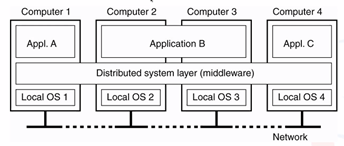
\includegraphics[width=110mm]{img/middle.png}
    \caption{Introduzione a SD}
    \label{fig:intro}
\end{figure}
\bigbreak
Definizione ironica di L.Lamport dei SD: sai che c'è un sistema distribuito quando il crash di un computer di cui non sapevi nulla, non ti permette di concludere il lavoro. 

\noindent Gli obbiettivi di un sistema distribuito sono:
\begin{enumerate}
    \item Accessibilità \\ Rendere le risorse sempre disponibili 
    \item Apertura \\ Un SD aperto è un sistema che offre servizi rispettando le regole standard che descrivono la semantica e rispettano la sintassi dei servizi stessi. Il rispetto di queste regole avviene mediante l'uso di interfacce scritte in IDL (Interface Definition Language) che descrivono il comportamento che il SD deve rispettare. E' molto utile in tutto il SW, questo garantisce interoperabilità, portabilità e estensibilità 
    \item Scalabilità \\ Un sistema può essere scalabile rispetto a:
    \begin{itemize}
        \item Dimensione: è possibile aggiungere utenti e risorse al sistema
        \item Geografico: utenti e risorse possono essere lontani
        \item Amministrazione: facilmente gestibile anche se copre strutture indipendenti
    \end{itemize}
    Possiamo avere problemi di scalabilità se usiamo:
    \begin{itemize}
        \item server centralizzati: avere un'unica macchina centrale rende il sistema non scalabile al crescere degli utenti
        \item Dati centralizzati: singola risorsa online per tutti gli utenti (all'inizio il servizio DNS era su un'unica macchina)
        \item Algoritmi centralizzati: routing con informazione completa del sistema. In un approccio decentralizzato non c'è una macchina che abbiamo una panoramica completa
    \end{itemize}
    \textit{Ex. sistema client-server: per renderlo scalabile potrei delegare parte del lavori di scripting lato client - validare il form - in alternativa, potrei duplicare la risorsa come per il DNS}
    \item Trasparenza \\ nascondere che il sistema è distribuito 
    \begin{figure}[h]
	\centering
    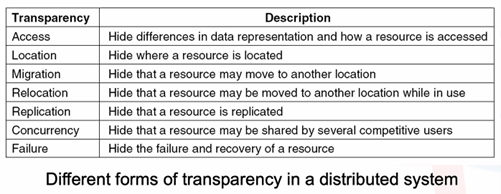
\includegraphics[width=110mm]{img/trasparenza.png}
    \caption{Diversi tipi di trasparenza in SD}
    \label{fig:trasparenza}
    \end{figure}
    \begin{itemize}
        \item Accesso: l'accesso ad un file condiviso da macchine diverse, con diverso SO e diverse rappresentazioni del file, dev'essere garantito senza usare primitive particolari. Solitamente si usano API standard
        \item Location: non devo sapere dove si trova la risorsa
        \item Migration: devo poter spostare una risorsa da una macchina all'altra (per manutenzione ad ex.) senza che l'utente se ne accorga
        \item Replication: potrebbe essere utile avere più copie di un file. Questo garantisce affidabilità in caso di guasti ed efficienza. Inoltre la dislocazione geografica potrebbe rendere più efficiente l'accesso alla risorsa e la dislocazione del carico. L'utente non deve sapere che la risorsa è duplicata
        \item Failure: il sistema deve nascondere i danni e gli errori e ripristinare automaticamente la risorsa. 
    \end{itemize}
\end{enumerate}

\noindent \textbf{Caratteristiche degli algoritmi decentralizzati:}
\begin{itemize}
    \item Nessuna macchina ha informazioni complete sullo stato del sistema
    \item Le macchine prendono decisioni su informazioni locali
    \item Il malfunzionamento di una macchina non comprometto l'intero sistema (no single-point-of-failure dell'approccio centralizzato)
    \item Non vengono fatte assunzioni riguardo all'esistenza di un orologio globale. Ciascun nodo ha un orologio e non sono mai sincronizzati perfettamente tra loro. 
\end{itemize}
Viene erroneamente assunto che in un SD:
\begin{itemize}
    \item La rete è affidabile
    \item La rete è sicura
    \item La rete è omogenea
    \item La topologia non cambia
    \item Assenza di latenza (impossibile non essendoci memoria condivisa i processi comunicano scambiandosi messaggi)
    \item La banda è infinita
    \item debuggare un'app distribuiti è come farlo per un'app standard.
\end{itemize}

\chapter{Sistemi distribuiti}
\label{cap:sistemi distribuiti}
Tipologia di sistema informatico costituito da un insieme di processi interconnessi tra loro in cui le comunicazioni avvengono solo tramite lo scambio di messaggi. Ogni nodo del sistema esegue un insieme di componenti che comunicano tra loro utilizzando uno strato software detto middleware che permette all'utente di percepire il sistema come un'unica entità. 
\section{Sistemi di calcolo distribuito:}
\label{sec:tipologie}
\begin{enumerate}
    \item Cluster
    \item GRID
    \item Cloud computing
    \item EDGE computing
\end{enumerate}

\subsection{Cluster}
\label{sec: cloud comp}
Collezione di macchine simili -solitamente con lo stesso SO - connesse da una rete locale LAN ad alta velocità. I sistemi cluster solitamente vengono usati per task che richiedono alte performance, disponibilità e affidabilità. \\ Ci sono due approcci diversi:
\begin{itemize}
    \item Approccio asimmetrico: esiste un nodo principale (master) che distribuisce i compiti ad un set di computer (Google Borg)
    \begin{figure}[h]
	\centering
    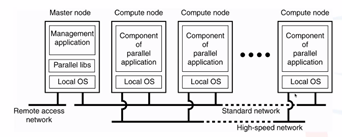
\includegraphics[width=90mm]{img/cluster.png}
    \caption{Ex. approccio asimmetrico}
    \label{fig:asimm}
    \end{figure}
    \item Approccio simmetrico: non c'è un nodo principale, è un sistema paritario in cui tutti i nodi ricoprono lo stesso ruolo. Comporta complicazioni perché questi nodi devono auto-organizzarsi per distribuire compiti e carico. 
\end{itemize}

\subsection{GRID}
\label{sec: grid}
Infrastruttura di calcolo distribuito, utilizzati per l'elaborazione di grandi quantità di dati, mediante l'uso di una vasta quantità di risorse (condivisione di risorse come CPU e dischi). Il GRID può essere visto come un super computer virtuale, composto da computer che agiscono insieme per eseguire compiti di grandi dimensioni, può essere percepito come un singolo sistema di un'organizzazione virtuale. Questi computer sono spesso eterogenei in termini di HW, SW, tecnologia di rete e SO. 
\bigbreak
La differenza tra cluster e GRID è che il cluster è una rete omogenea in cui i dispositivi hanno gli stessi componenti HW e lo stesso SO connessi insieme in un cluster mentre il GRID è una rete eterogenea in cui i dispositivi possono variare.

\subsection{Cloud computing}
\label{sec: cloud}
Modello per avere un accesso alla rete onnipresente, conveniente, on-demand per condividere pool di risorse di computazione configurabili (rete, server, storage, applicazioni) che può essere richiesta o rilasciata con uno sforzo minimo di gestione e senza l'intervento del provider. Necessitano di speciale tecnologia di commutazione e bilanciamento del carico. \\ Caratteristiche del cloud:
\begin{itemize}
    \item Nodi eterogenei in HW e SW
    \item Connessioni di rete eterogenee in capacità e affidabilità
    \item On demand self-service: capacità di riorganizzare le risorse date agli utenti in modo automatico
    \item Ampio accesso alla rete
    \item Resource Pooling: il fornitore delle risorse gestisce più clienti
    \item Elasticità e rapidità nel fornire o rilasciare risorse
    \item Sistemi di misurazione: i cloud controllano e ottimizzano l'uso delle risorse. 
\end{itemize} 
\noindent Modelli del cloud:
\begin{itemize}
    \item SaaS (Software as a Service): uso l'applicazione del fornitore che gira su un'infrastruttura cloud (non sono interessato a scaricare SW, GMAIL o Microsoft Office 365). 
    \item PaaS (Platform as a Service): rilascio sull'infrastruttura di applicazioni create dal consumer usando tool supportati dal fornitore. Voglio sviluppare l'applicazione finale (algoritmo per image recognition o videogame) ma vorrei usare un DB ad alte  performance.
    \item IaaS (Infrastructure as a Service): rilascio ed esecuzione di SW arbitrario (compreso SO e applicazioni) sull'infrastruttura cloud. E' come chiedere una macchina completa per poter sviluppare e implementare quello che l'utente desidera. 
\end{itemize}
\bigbreak
\noindent Modelli di rilascio del cloud:
\begin{itemize}
    \item Private Cloud: esclusivo per una singola organizzazione 
    \item Community Cloud: diverse organizzazioni insieme
    \item Public Cloud: ad uso aperto
    \item Hybrid Cloud: combinazioni di una o più modelli di rilascio del cloud. 
\end{itemize}
La differenza tra cloud computing e cluster computing: il cloud è una tecnologia che fornisce molti tipi di risorse come servizi, soprattutto su internet, mentre il cluster computing si concentra su prestazioni migliori e disponibilità di un servizio collegando una collezione di macchine stand-alone per formare una singola risorsa di calcolo integrata. I cluster sono principalmente utilizzati per il bilanciamento del carico e per fornire un'elevata disponibilità (un singolo carico di lavoro, un calcolo, viene condiviso da diversi computer collegati tra loro, che funzionano come una singola entità), mentre il cloud si concentra sulla fornitura di servizi come SW, piattaforme. Ma una cosa importante da notare è che il cloud è costruito in base a un cluster di server. 


\subsection{EDGE computing}
\label{sec: EDGE}
Modello di calcolo distribuito nel quale l'elaborazione dei dati avviene il più vicino possibile a dove i dati vengono richiesti. Solitamente è contrapposto all'elaborazione centralizzata tipica del cloud computing. Processare i dati ai margini, vicino al luogo dove sono generati, porta considerevoli vantaggi in termini di latenza di elaborazione, riduzione di traffico dati. Questo modello è adottato nell'IoT, questo fa un largo uso di sensori che producono una grande mole di dati con esigenza di processing real-time. I device EDGE comunicano con questi device, eseguendo i calcoli richiesti con bassa latenza e rispettando esigenze real-time. 

\section{Sistemi transazionali o pervasivi}


\subsection{Sistemi di elaborazione delle transazioni}
\label{sec:sist trans}
Il termine transazione indica una qualunque sequenza di operazioni lecite che causa un cambiamento nello stato di un DB. \\ Le transazione rispetta le proprietà ACID:
\begin{itemize}
    \item Atomiche: la transazione è indivisibile per il mondo esterno
    \item Consistenti: quando la transazione inizia il DB si trova in uno stato coerente, quando la transazione finisce il DB dev'essere in uno stato coerente
    \item Isolate: transazioni concorrenti non devono interferire tra loro
    \item Durature: una volta resa effettiva la modifica, dev'essere permanente
\end{itemize}

\subsection{Sistemi distribuito pervasivo}
\label{sec:pervasiv}
E' un sistema formato da nodi eterogenei, tra i quali ci sono anche nodi non convenzionali (solitamente mobili come smartphone, IoT, sensori), questi sono oggetti con capacità di computazione e memoria ridotta. Sono reti "challenged" poiché sono reti instabili e mutevoli: i nodi si possono muovere, cambiare rete, la topologia di rete cambia spesso. Inoltre un sistema distribuito pervasivo deve considerare il contesto e adattare il comportamento nell'ottica di ottimizzare gli obbiettivi del sistema. 

\chapter{Architetture}
\label{cap:arch}
L'architettura di un SD definisce:
\begin{itemize}
    \item entità principali del sistema: quali sono i processi o thread che girano sui nodi, quali sono i nodi sensori e attuatori nei sistema pervasivi, gli oggetti e le componenti. 
    \item pattern di comunicazione: decido come comunicano le entità, se usare publish/subscribe o socket o P2P ad esempio.
    \item comunicazione: come le entità comunicano anche se sono dislocate in posti diversi
    \item come le entità vengono mappare nell'infrastruttura fisica - replicazione, clustering, caching 
\end{itemize}

\section{Stili architetturali}
\begin{itemize}
    \item Architettura a livelli: permette di astrarre dai particolari che caratterizzano i livelli inferiori e permette di separare funzionalmente le componenti del sistema delegando a ciascun livello un compito specifico (approccio già usato per TCP/IP). 
    \item Architetture basate sugli oggetti: rappresenta ogni componente del sistema come un oggetto, ogni oggetto mette a disposizione dei metodi (remoti) visibili e richiamabili dagli oggetti (CORBA)
    \item Architetture centrate sui dati: stile in cui le componenti usano uno spazio di dati condiviso per interagire tra di loro (FS distribuiti)
    \item Architettura basate su eventi: il middleware deve gestire la comunicazione tra le varie componenti che avviene tramite occorrenza di eventi. Ogni componente interessato ad un evento viene notificato ogni volta che esso si verifica (Publish-subscribe). 
\end{itemize}

\section{Tipi di architettura}
\begin{enumerate}
    \item Architetture centralizzate
    \item Architetture decentralizzate
    \item Architetture ibride
\end{enumerate}

\subsection{Architetture centralizzate}
\begin{itemize}
    \item Client- server (request/response pattern)
    \item Event Bus Architecture (publish/subscribe pattern)
\end{itemize}
Il modello base è quello in cui vi è interazione tra un componenti che richiede un servizio (client) e l'altro componente che risponde (server). L'interazione avviene stabilendo un canale di comunicazione tra le parti (anche a questo punto tipo di architettura è possibile applicare uno stile a livelli, ad ex. un motore di ricerca ha un livello di interfaccia utente, un livello applicativo e uno di gestione dei dati). 
\bigbreak
\noindent Distribuzione verticale: diverse funzionalità vengono assegnate a componenti diversi del sistema 
\bigbreak
\noindent Distribuzione orizzontale: la stessa funzionalità è distribuita tra più componenti del sistema (replica di web service). 
\bigbreak
\noindent \textbf{Modello client-server} 
\bigbreak
Processo server in esecuzione su un nodo e più processi client in esecuzione su altri. Viene istituito un canale tramite il quale il client manda richieste al server. Il server gestisce richieste concorrenti e risponde a tutti

\begin{figure}[h] 

3 warnings

     \centering
     \begin{subfigure}[b]{0.3\textwidth}
         \centering
         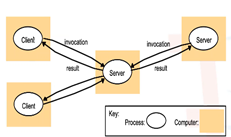
\includegraphics[width=60mm]{img/cs.png}
         \caption{Modello client-server}
     \end{subfigure}
     \hfill
     \begin{subfigure}[b]{0.5\textwidth}
         \centering
          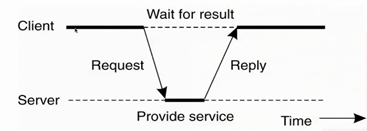
\includegraphics[width=60mm]{img/cs2.png}
          \caption{Interazione client-server}
     \end{subfigure}
    \caption{Approccio centralizzato}
    \label{fig:acc}
\end{figure}

La questione è cosa far eseguire lato client e cosa lato server. Posso fare quasi tutto lato server - il client è in grado solo di visualizzare immagini, viene confezionato tutto dal server e mandato al client. Posso usare una via di mezzo, effettuando una parte di interpretazione scripting lato client con Javascript. All'estremo opposto posso avere tutto lato client ed eseguire query al DBMS verso il server. 
\bigbreak
\noindent \textbf{Event Bus Architectur - publish/subscribe} \\

\begin{figure}[h]
\centering
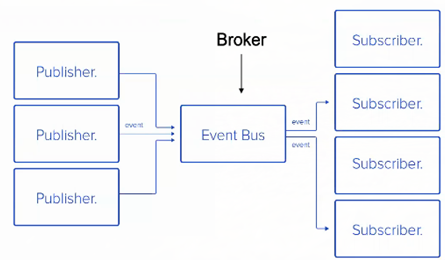
\includegraphics[width=90mm]{img/ppsub.png}
\caption{publish-subscribe}
\label{fig:psub}
\end{figure}
Questa architettura è composta da server, chiamati publisher, che comunicano il verificarsi di un evento (ad ex. un publisher ha montato un sensore per la temperatura ed ogni 10s manda un aggiornamento) e da client, chiamata subscriber, che sottoscrivono uno specifico evento dichiarandosi interessati a ricevere aggiornamenti (ad ex. sono interessato alle temperature). Componenti essenziale è l'Event Bus, gestito da un componente software: il Broker. Il broker media tra le due componenti sopra: riceve le sottoscrizioni dai subscriber e gli aggiornamenti dei publisher. Il broker ha un DB nel quale mantiene le sottoscrizioni ai vari canali, il broker ha il compito di comunicare ai subscriber gli aggiornamenti riguardanti gli eventi a cui sono interessati. \textbf{La comunicazione è asincrona}.
\newpage
\subsection{Architetture decentralizzate}
\bigbreak
\noindent \textbf{Modello Peer-to-Peer} 
\bigbreak
In un modello P2P puro ogni nodo ha le stesse capacità (stesso codice su ogni macchina), il sistema è progettato in modo che le risorse gestite da ogni peer debbano essere condivise. Le operazioni non dipendono da alcun coordinatore (non c'è load balancer e distribuzione orizzontale client/server). \\ Esempio di P2P: Napster. Napster non è un P2P puro in quanto c'è un server che contiene un indice, se un peer A vuole una risorsa, fa una richiesta al Napster server. Quest'ultimo non possiede direttamente la risorsa, ma sfruttando l'indice, indirizza il peer A verso i peer che la possiedono. A questo punto il peer A domanda la risorsa al peer B che la possiede, il peer B si comporta da server fornendo il file richiesto. In ultima cosa il peer A, ottenuta la risorsa, comunica al server di aggiornare l'indice in modo che sia al corrente che anche lui possiede la risorsa ora. \\ Questioni nella distribuzione di risorse su molti host:
\begin{itemize}
    \item Raggiungere bilanciamento del carico
    \item Assicurare disponibilità di risorse limitando sovraccarichi e limitando traffico inutile
\end{itemize}
Ci sono 3 generazioni di P2P:
\begin{enumerate}
    \item Sistemi di condivisione file (Napster - anni 90')
    \item Cercando di superare i limite di Napster (scalabilità, resistenza ai guasti, anonimità) nascono: Gnutella, FreeNet, bitTorrent
    \item P2P middleware: si vuole permettere ai client, i programmatori che usano il middleware) - in modo trasparente - di localizzare le risorse e comunicare con i nodi della rete. Questi sistemi devono essere dinamici, cioè devono permettere di aggiungere nuove risorse e aggiungere nuovi nodi. Si cerca di ottmizzare la scalabilità, efficienza, bilanciamento del carico, anonimità. ex. Pastry, Tapestry, Chord, CAN. \\ Per fare questo vengono costruite delle \textbf{overlay network}
\end{enumerate}

\section{Overlay network}
Le overlay network sono reti virtuali costruite sulle reti reali che uniscono i peer. L'instradamento dei messaggi avviene tramite un algoritmo indipendente dalla costituzione della rete sottostante. Questo significa che l'instradamento, oltre ad avvenire a livello rete, avviene anche a livello applicazione (il routing avviene a livello logico e non fisico). Useremo questa rete logica per fare in modo efficiente quanto abbiamo detto sopra: gestire risorse, aggiunge e rimuovere nodi e risorse. 

\noindent \textbf{Routing overlay}: il SW della rete logica deve fare routing delle richieste dai client agli host che contengono le risorse d'interesse. Questo routing è fatto a livello applicazione e non a livello rete, esso è infatti basato su ID globali delle risorse nel SD e dev'essere diretto ai peer che contengono repliche di quella risorsa. Il routing overlay deve anche occuparsi dell'aggiunta e della rimozione di peer dalla rete. \\ Ci sono due tipologie di reti logiche:
\begin{enumerate}
    \item Strutturata
    \item Non strutturata
\end{enumerate}

\subsection{Reti logiche strutturate}
Sono le maggiormente usate perché danno garanzie maggiori. La rete logica viene costruita in modo deterministico utilizzando una DHT (Distributed Hash Table). L'obbiettivo è l'instradamento efficiente al nodo che contiene i dati. Ogni peer conosce l'intera struttura della rete
\bigbreak
\noindent \textbf{CHORD} 
\begin{figure}[h]
\centering
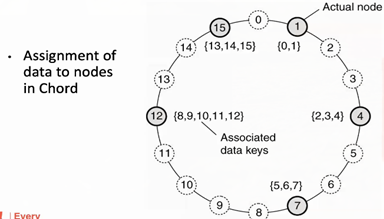
\includegraphics[width=70mm]{img/chord.png}
\caption{CHORD}
\label{fig:chord}
\end{figure}

\noindent E' un sistema basato su tabelle di hash distribuite e un anello logico. \\
Viene fissato uno spazio di indirizzamento (in figura $2^4$ bit) e c'è una funzione di hash che - per ogni nodo e risorsa - assegna un ID. 
\begin{itemize}
    \item ID(node) = hash(IP, porta)
    \item ID(key) = hash(key)
\end{itemize}
Per assegnare l'ID ad un nodo, la funzione di hash prende in input l'indirizzo IP della macchina e il numero di porta del processo e ridà in output un indirizzo nello spazio definito prima. Lo stesso spazio di indirizzamento vale per la creazione degli ID per le risorse, in input viene preso il nome, il titolo della risorsa. \\ Dobbiamo a questo punto capire come assegnare le risorse ai nodi? \\ Una volta assegnato un ID ad una risorsa, se ne occuperà il più vicino nodo successore. 
\bigbreak
Supponiamo di avere una risorsa con ID \textit{k}, essa viene mappata nel nodo con $ID >= k$. Questo procedimento viene detto \textbf{successore di k} (una risorsa con $ID = 3$ viene assegnata al nodo 4, se il nodo 4 esiste ed è attivo). \\
La problematica maggiore è fare \textit{succ(k)}: quando viene richiesta una risorsa ad un nodo, il nodo manda un messaggio di ricerca. Esso ha un puntatore in avanti e uno indietro verso i nodi vicini, l'algoritmo ha una complessità lineare nel numero di nodi - non è molto efficiente
\bigbreak
Vorrei migliorare la situazione, usando un algoritmo con complessità logaritmica nel numero di nodi - uso tabelle di hash distribuite (DHT). Ogni nodo attivo ha una sua struttura dati locale, finger table, la tabella di hash. Risultano distribuite perché sono tante piccoli parti di una tabella di hash distribuite nell'anello. 
\begin{figure}[h]
\centering
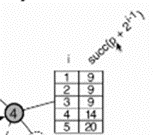
\includegraphics[width=30mm]{img/chordh.png}
\caption{Esempio tabella di hash in un nodo}
\label{fig:chorddh}
\end{figure}
\bigbreak
Ogni nodo conosce \textit{n} vicini e la distanza tra sé e i nodi che conosce, cresce esponenzialmente.

\begin{figure}[h]
\centering
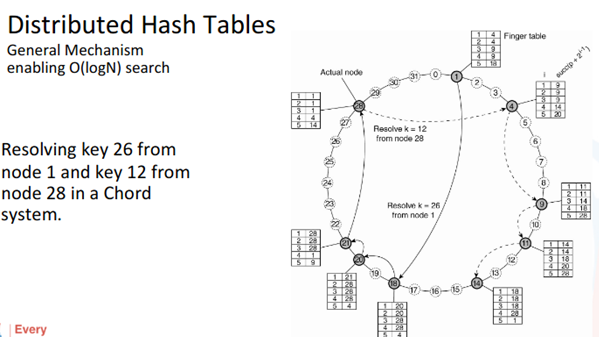
\includegraphics[width=60mm]{img/compitochord.png}
\caption{Compito chord}
\label{fig:chorddh}
\end{figure}

\bigbreak
\noindent \textbf{CAN}
\begin{figure}[h]
\centering
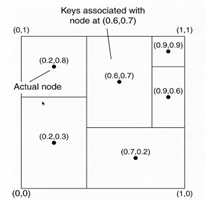
\includegraphics[width=60mm]{img/can.png}
\caption{CAN}
\label{fig:can}
\end{figure}
Sistema basato su tabelle di hash distribuite e su uno spazio cartesiano d-dimensionale. Questo spazio viene partizionato e ciascuna regione è assegnata ad un nodo, questi nodi gestiscono tutte le risorse che vengono mappate nella loro regione di appartenenza. \\ Ogni chiave dei dati è un punti, ogni nodo gestisce i punti mappati nella sua regione. \\ Per permettere l'arrivo di un nuovo nodo, l'area viene divisa in due sotto-regioni. Meno immediata è la rimozione del nodo: non è sempre possibile creare un rettangolo dall'unione di due rettangoli.

\subsection{Reti logiche non strutturate}
La rete è costruita mediante l'utilizzo di algoritmi randomici. 

Ogni nodo non conosce tutto il resto della rete, ha una conoscenza locale. Se non possiede una risorsa, propagherà la richiesta ai nodi conosciuti. La rete logica viene creata mediante lo scambio di viste (la conoscenza che ha ogni peer è parziale). \\ Il routing è basato su:
\begin{itemize}
    \item [--] Ogni nodo memorizza una lista di nodi vicini costruita casualmente (view)
    \item [--] La lista parziale è aggiornata ogni tanto, questo avviene tramite protocolli di gossiping: nodi vicini si scambiamo informazioni su nodi nuovi che hanno conosciuto. C'è una componente random perchè viene scelta una percentuale a caso della view conosciuta da un nodo.
    \item [--] Anche le risorse sono spesso assegnate in modo randomico ai nodi
    \item [--] La ricerca di risorse quindi non può restituire upper-bound né può garantire che la risorsa venga trovata se presente nel sistema. La ricerca è spesso limitata, parto una certo nodo, se questo non la possiede, chiede ai suoi vicini e via così. C'è un limite di tempo dato da un timeout o da un numero massimo di hop per limitare overhead. 
    \item [--] Manutenzione non impegnativa e migliore scalabilità
    \item [--] Spesso vi è una struttura gerarchica: per problemmi di scalabilità a volte vi sono nodi che sono visti come superpeer in quanto svolgono funzioni differenti dai normali peer (Directory server di Napster). 
\end{itemize}

\begin{figure}[h]
\centering
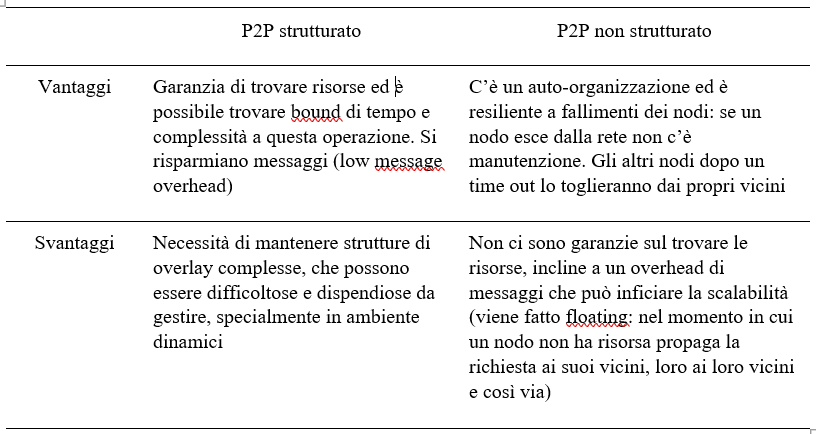
\includegraphics[width=130mm]{img/proscos.PNG}
\caption{Vantaggi e svantaggi strutturato/non strutturato}
\label{fig:vssn}
\end{figure}

\subsection{Architetture ibride}
Sono architetture parzialmente centralizzate e parzialmente decentralizzate. 
\bigbreak
\noindent \textbf{Superpeer}: ci sono nodi con funzionalità maggiori che gestiscono un certo sotto insieme di peer
\bigbreak
\noindent \textbf{Sistemi distribuiti collaborativi}: sistemi che utilizzano peer per scambiare dati, ma che gestiscono il bootstrapping usando il protocollo client-server
\bigbreak
\noindent \textbf{Bit torrent}: è un’architettura P2P ma non è pura: spesso c’è una componente iniziale in cui troviamo qualcosa che aiuta – in modo centralizzato – ad orientarsi nella rete. \\
Un client chiede ad un web server, che ridà un file .torrent che restituisce l’indirizzo di un tracker del file che contiene la lista dei nodi che hanno a disposizione il file.
C’è un inizio di client server e poi P2P (sistema ibrido)

\section{Micro-servizi}
Raffinamento o caso particolare della distribuzione verticale delle funzionalità: voglio isolare maggiormente le singole funzionalità, rendendole ciascuna indipendente dalle altre. Ogni componente/funzionalità dell'applicazione logica dev'essere in un processo separato, se possibile in una macchina separata. I micro-servizi devono essere aggiornabili e rimpiazzabili indipendentemente dagli altri, perciò sono "impacchettati" con tutti i package necessari al loro  funzionamento. \\  Chiaramente esse dovranno coordinarsi, quindi comunicare tra loro. Per farlo utilizzano meccanismi di comunicazione leggera (REST API o RPC). \\ I micro-servizi hanno avuto successo con i SD e i cloud perché la replicazione di funzionalità su più server è resa più semplice: ho bisogno che un componente sia replicato molte più volte di un altro. Con un'architettura monolitica ho tutte le funzionalità in un server, quando lo replico copio l'intero server con tutte le funzionalità al suo interno. 

\begin{figure}[h]
\centering
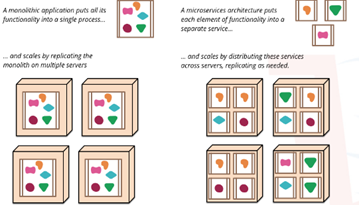
\includegraphics[width=130mm]{img/microser.png}
\caption{micro-servizi}
\label{fig:ms}
\end{figure}

\section{Containers}
Astrazioni – nel layer applicativo – che mettono insieme il codice e le dipendenze (quando sviluppo un applicativo esso userà della librerie oppure una specifica versione di un DB. Quando devo migrare il mio applicativo su un altro server non è detto che esso abbia tutte le dipendenze che mi servono, porting da incubo).
\begin{itemize}
    \item [--] si vuole offrire supporto per l'architetture a micro-servizi
    \item [--] si vuole incrementare portabilità SW, facilità di migrazione
    \item [--] si vogliono ridurre i problemi si presentano durante lo sviluppo
\end{itemize}
\begin{figure}[h]
\centering
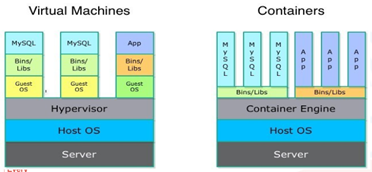
\includegraphics[width=130mm]{img/container.png}
\caption{containers}
\label{fig:conta}
\end{figure}
I container non sono una macchina virtuale, essi virtualizzano solamente l’applicazione e tutte le librerie da cui dipende anziché l’intero SO, mettendo un container engine (ad es. Docker) sopra il layer del SO della macchina host. Il risultato è che il container è molto più leggero di un VM, e permette una portabilità maggiore in quanto non è limitato dal SO. I container non sono un SD, in quanto girano su un’unica macchina. L’idea è quella di avere un SD in cui ogni nodo ha una versione del container engine, con un nodo che fa da coordinatore decidendo quali container ci sono su ogni nodo. \\
Ex. Kubernetes: piattaforma pensata per mantenere e gestire containers su dei cluster, facilitandone la configurazione dichiarativa e automazione. I componenti di un'applicazione sono detti pods, ogni cluster ha dei lavoratori che fanno da host per i pods.

\chapter{Modelli di comunicazione}
\label{cap:mod comm}
Servono perchè un SD funziona tramite scambi di messaggi tra processi in esecuzione su nodi diversi, eterogenei e distribuiti geograficamente. Questo insieme di nodi è collegato da una rete. \\ Distinguiamo la comunicazione in base a :
\begin{itemize}
    \item Persistente/Transiente
    \item Sincrono/Asincrono
\end{itemize}

Tipologie di comunicazione:
\begin{enumerate}
    \item Berkeley Socket: comunicazione transiete, tipicamente sincrona orientata al messaggio
    \item RPC (Remote Procedure Call)
    \item Sistema a code e message broker: comunicazione persistene, asincrona basata sui messaggi
    \item Data streams
\end{enumerate}

\begin{figure}[h]
\centering
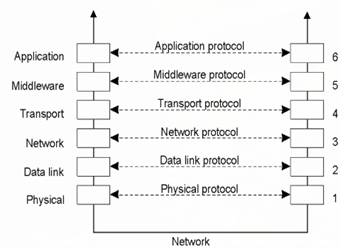
\includegraphics[width=130mm]{img/middl.png}
\caption{Layer middleware}
\label{fig:middlelayer}
\end{figure}
Simile al modello ISO/OSI ma mancano layer di sessione e presentazione che sono fusi nel middleware (lavoriamo sempre dal livello di trasporto in su in questo corso). \\ I servizi di comunicazione citati sopra sono collocati nel layer di middleware: i protocolli middleware sono un sistema di protocolli che definiscono servizi utili per un ampio spettro di applicazione. 
\bigbreak
\noindent \textbf{Sistema di comunicazione persistente}
\noindent La comunicazione avviene anche quando il destinatario non è presente. Un esempio nella vita reale è il pony express: infrastruttura di fondo rappresentata dagli ufficio postali e i pony spostano i messaggi da un posto all'altro. \\ Ci sono due tipi:
\begin{itemize}
    \item Asincrona: il processo A non si ferma in attesa della risposta di B, sarà compito del middleware memorizzare il messaggio fino a che B non è operativo
    \item Sincrono: il processo A si ferma quando invia il messaggio in attesa di una risposta dal processo B. Nel processo B è implementato un sistema di memorizzazione che immagazzina i dati nel caso in cui l'applicazione non sia ora disponibile. Inoltre invia una notifica al processo mittente per permettergli di sbloccarsi. 
\end{itemize}
\bigbreak
\noindent \textbf{Sistema di comunicazione transiente}
Non c'è modo di memorizzare messaggi in transito, se il processo destinatario non è disponibile la comunicazione fallisce. Ex. provare a chiamare un amico che non può rispondere al telefono in quel momento. \\ Ci sono varianti:
\begin{itemize}
    \item Asincrona: il processo A invia un messaggio a B e continua la sua esecuzione. Quando il processo B riceve il messaggio non deve inviare nulla ad A
    \item Sincrona basata su ricezione: il processo A invia il messaggio a B e si ferma, il processo B invia un ACK ad A quando ha ricevuto il messaggio e quando ha tempo, esegue la richiesta
    \item Sincrona basata su consegna: il processo A aspetta finché il messaggio non è in elaborazione da B
    \item Sincrona basata su risposta (esecuzione): il processo A aspetta fino a che B non finisce di elaborare la sua richiesta. 
\end{itemize}
In generale, se la consegna non è possibile, il messaggio viene eliminato. E' una tipica comunicazione a livello trasporto: i router memorizzano ed inoltrano, ma cancellano se non è possibile inoltrare. 
\bigbreak
\noindent \textbf{Sistema di comunicazione sincrona}
\noindent Una volta sottomesso il messaggio, il mittente si blocca finchè l'operazione non è completata. 
\begin{itemize}
    \item invio e ricezione sono operazioni bloccanti
    \item mittente è bloccato fino a quando il middleware non prende il controllo della trasmissione oppure fino a che il messaggio non è ricevuto/elaborato dal destinatario 
\end{itemize}

\bigbreak
\noindent \textbf{Sistema di comunicazione asincrona}
\noindent Una volta inviato il messaggio, il processo mittente continua l'elaborazione: il messaggio  viene posto in coda in attesa che il ricevente lo accetti - senza che il mittente rimanga bloccato in attesa dell'ACK. 
\begin{itemize}
    \item invio è operazione non bloccante
    \item ricezione può essere bloccante o non bloccante
\end{itemize}

\noindent Esempi:
\begin{itemize}
    \item persistente e asincrono
    \begin{figure}[h]
    \centering
    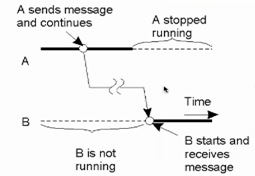
\includegraphics[width=45mm]{img/comm1.png}
    \end{figure}
    \bigbreak
    Il processo A vuole comunicare con B, il processo B non è in esecuzione. Le ondine rappresentano un sistema di memorizzazione intermedia, questo garantisce persistenza. Il fatto che A continui l'esecuzione dopo l'invio del messaggio ci dice che è una comunicazione asincrona. 
    
    \item persistente e sincrono
    \begin{figure}[h]
    \centering
    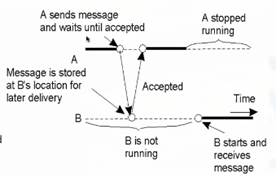
\includegraphics[width=45mm]{img/comm2.png}
    \end{figure}
    
    Il processo A manda un messaggio a B, che non è in esecuzione, ma accetta comunque il messaggio. Questo ci dice che il sistema è persistente. Il processo A manda il messaggio è si blocca fino all'arrivo di un ACK in cui è specificato che il messaggio è stato accettato da B (non necessariamente processato) . Questo ci dice che il sistema è sincrono
    
    \item transiente e asincrono
     \begin{figure}[h]
    \centering
    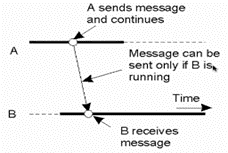
\includegraphics[width=45mm]{img/comm3.png}
    \end{figure}

    Il processo A invia il messaggio e continua l'esecuzione, il sistema è asincrono. Non ci sono componenti intermedi che memorizzano il messaggio, se B non è attivo il messaggio è perso. Questo ci dice che il sistema è transiente.
    
    \item transiente, sincrono, receipt-base
     \begin{figure}[h]
    \centering
    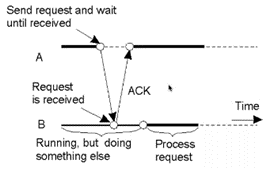
\includegraphics[width=45mm]{img/comm4.png}
    \end{figure}

    Il processo A manda un messaggio e aspetta la risposta, è sincrono. Non ci sono livelli intermedi di memorizzazione, è transiente. E' receipt-base perché il processo A attende un ACK quando il processo B riceve il messaggio, non gli interessa sapere se l'ha processato
    
    \item transiente, sincrono, delivery-based
     \begin{figure}[h]
    \centering
    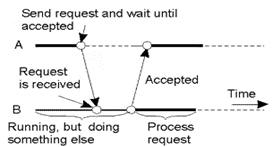
\includegraphics[width=45mm]{img/comm5.png}
    \end{figure}
    
    In questo caso è delivery-based perchè il processo A attende un ACK per sapere se il messaggio viene processato, non gli basta sapere che B l'ha ricevuto
    
    \item transiente, sincrono, response-based
     \begin{figure}[h]
    \centering
    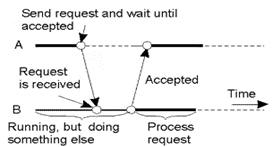
\includegraphics[width=45mm]{img/comm5.png}
    \end{figure}
    \\
    Il processo A è bloccato fino a quando non riceve il risultato della richiesta inviata al processo B (ex. RPC: il processo A non è in grado di eseguire calcolo di matrici, il processo A manda i dati al processo B e deve aspettare che B gli restituiscano il risultato per continuare)
\end{itemize}

\section{Berkeley Socket}
Comunicazione transiente orientata ai messaggi. \\
Collegamento virtuale che unisce un processo su un nodo ad un altro processo su un altro nodo. Per aprire una connessione tra due nodi, entrambi devono chiamare la primitiva socket e aprire una socket. 

\begin{figure}[h]
\centering
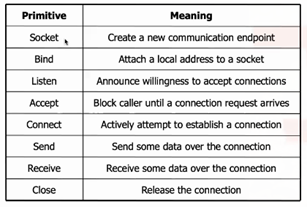
\includegraphics[width=70mm]{img/socket.png}
\end{figure}
Dal punto di vista del SO questo crea uno spazio di memoria e un descrittore (quando un processo pare un file, il SO assegna un descrittore (un numero) a quel file, in modo da poter richiamare il file "read desc" o "write desc"). \\ Una volta lanciata la primitiva socket, anche ad essa è assegnato un descrittore dandole il primo numero disponibile (0, 1, 2 sono descrittori di sistema, supponiamo le venga assegnato 4. Da ora fare "write 4" si riferisce alla socket creata). 

Una volta creata la socket, essa deve raggiungere anche l'altro terminale di comunicazione tramite la pila di protocollo di rete. Un terminale è ovviamente indirizzato usando IP, ma vorrei parlare con uno specifico processo eseguito su quel server, per questo viene usato anche il numero di porta. Devo poter fornire un indirizzo più generale a TCP/IP (il descrittore assegnato alla socket dalla macchina è locale). Viene chiamata la primitiva bind, un indirizzo locale di una macchina è una porta (il descrittore 4 viene assegnato ad una porta).

\begin{figure}[h]
\centering
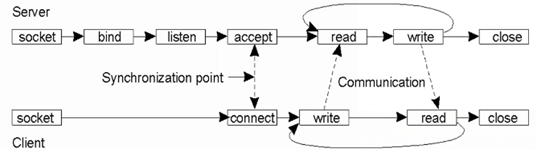
\includegraphics[width=80mm]{img/fasi socket.png}
\end{figure}

La primitiva listen serve tipicamente al server per esprimere la disponibilità ad iniziare la comunicazione. La primitiva accept accetta effettivamente la comunicazione. La primitiva connect viene eseguita dal client (passa IP e porta del server), che chiede di connettersi al server. In ultimo viene chiamata la primitiva close, il sistema funziona anche senza, ma così rilascio risorse. 
\bigbreak
Il modello della socket è transiente: il server esegue un accept per accettare connessioni da parte del client che esegue una connect. Il client deve trovare dall'altra parte il server pronto ad eseguire le richieste (se non lo trova non viene stabilito canale di comunicazione). 

\section{Sistemi a code}
Comunicazione persistente orientata agli oggetti \\

\begin{figure}[h]
\centering
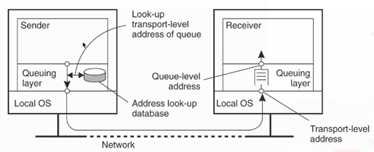
\includegraphics[width=80mm]{img/code1.png}
\end{figure}
Tra processo mittente e destinatario ci sono diversi nodi che gestiscono i messaggi: nel caso il ricevente non sia disponibile, i nodi intermedi - che formano il livello middleware - memorizzano il messaggio fino a che il ricevente non torna disponibile.
\bigbreak
Il SO ha un punto di comunicazione che è un punto di accesso alle code (prima leggeva e scriveva sulla socket). L'applicazione del mittente A manda il messaggio a una coda, la quale fa riferimento al sistema di routing intermedi e il messaggio arriva all'applicazione del destinatario che legge da una coda. 

\begin{figure}[h]
     \centering
     \begin{subfigure}[b]{0.3\textwidth}
         \centering
         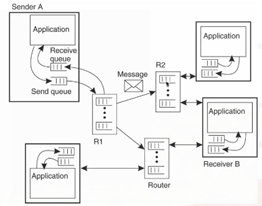
\includegraphics[width=60mm]{img/code2.png}
     \end{subfigure}
     \hfill
     \begin{subfigure}[b]{0.5\textwidth}
         \centering
          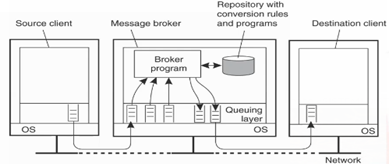
\includegraphics[width=60mm]{img/code3.png}
     \end{subfigure}
\end{figure}
Message broker: colui che si occupa di ridirigere i messaggi nelle code di appartenenza, garantendo persistenza, permettendo inoltre la conversione in una formato comprensibile dai nodi. \\
Quando uso un sistema a code?
\begin{itemize}
    \item mi serve comunicazione asincrona ma persistente
    \item ammetto dei ritardi e posso implementare scalabilità
    \item il produttore è più veloce del consumatore (sensore che produce dati ambientali e consumatore non riesce a gestirli tutti)
    \item si implementa un patteren di comunicazione publish-subscribe
\end{itemize}

\section{Remote Procedure Call}
RPC si riferisce all'attivazione da parte di un programma di una procedura attivata su una macchina diversa da quella sulla quale il programma viene eseguito. 
\bigbreak
Il concetto di RPC è definito come meccanismo sincrono: il processo di comunicazione tramite RPC prevede il passaggio di parametri e restituzione di un valore di funzione.

Idealmente il programmatore non dovrebbe preoccuparsi della procedura di chiamata, dovrebbe essere di facile attuazione come le chiamate di procedura locali (trasparenza). 

L'implementazione di una RPC comporta lato mittente delle istanze particolari, chiamati \textbf{stub}
\bigbreak
RPC standard \textit{read(fd, buffer, nbytes)} 
\begin{itemize}
    \item fd: file descriptor
    \item buffer
    \item nbytes: totale numero di bytes da leggere
\end{itemize}

\begin{figure}[h]
\centering
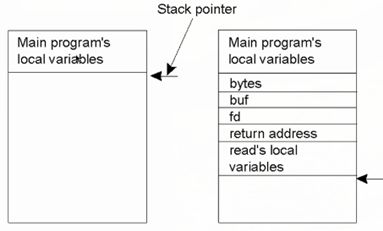
\includegraphics[width=80mm]{img/rpc.png}
\end{figure}
\noindent sx: stack di esecuzione. Quando chiamiamo la procedura allochiamo spazi di memoria dove mettiamo i parametri. C'è un problema nel passaggio dei parametri per rendere remota questa chiamata. Posso passare i parametri per valore o per riferimento (puntatore), il problema nasce nel passaggio per riferimento in quanto un processo remoto in esecuzione su un'altra macchina non ha visibilità della memoria del chiamante (sono indirizzi locali al processo mittente).
\\ Devo passare i valori e il server crea la struttura dati per contenere tutto, quando risponde al client non potrà farlo usando indirizzi locali, userà sempre un valore (fase di serializzazione). E' il middleware che si occupa di serializzare in modo che il programmatore non se ne debba preoccupare. 

\begin{figure}[h]
\centering
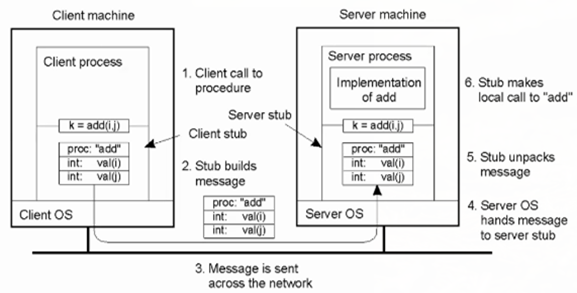
\includegraphics[width=80mm]{img/rpc2}
\end{figure}

\noindent Fasi di una RPC:
\begin{enumerate}
    \item Il client chiama la procedura remota, a questo punto interviene un pezzo di codice non scritto dal programmatore ma automaticamente generato - cient stub
    \item Lo stub impacchetta la RPC, costruisce il messaggio e serializza i parametri comunicando con il SO locale
    \item Il SO manda il messaggio, opportunamente formattato dal client stub, al server stub tramite la rete. 
    \item Il messaggio arriva al processo server che si è reso disponibile ad eseguire la procedura (il server ha codice scritto al suo interno che permette di eseguire quella specifica procedura, l'implementazione è scritta per essere eseguita in locale senza preoccuparsi di risponde a chiamate da remoto).

\noindent Il SO del server riceve il messaggio e lo passa al server stub:

    \item Il server stub spacchetta il messaggio, identifica la funzione all'interno e crea una struttura dati se necessario
    \item Il server stub esegue una chiamata alla funzione verso il server, come se fosse una chiamata locale
    \item Il server stub impacchetta il messaggio e lo passa al SO
    \item Il messaggio è inviato, tramite la rete, al client stub. Lo stub del client spacchetta la risposta e la restituisce al client
\end{enumerate}
Il server per pubblicare metodi remoti deve scrivere in un linguaggio neutro per definire l'interfaccia di comunicazione (dev'essere scritta in IDL - Interface Definition Language). Parto da un IDL comune, poi c'è un compilatore che compila nei vari linguaggi.
\bigbreak
\noindent \textbf{Marshalling e Unmarshalling}
Processo compiuto dallo stub. Il marshalling consiste nel formattare i parametri della chiamata in un messaggio (serializzarli e metterli nel messaggio). Questo richiede la serializzazione di oggetti o strutture dati. Se abbiamo nodi eterogenei è possibile che interpretino i dati in modo diverso: il passaggio per valore va bene ma attenzione alla rappresentazione
\bigbreak
\noindent \textbf{RPC sincrono e asincrono}
Tipicamente RPC è sincrona (resta in attesa della risposta della procedura remota). Esiste un metodo in cui posso richiedere una RPC asincrona: posso aspettare un ACK che dice se la richiesta di esecuzione della chiamata è stata ricevuta. \\ Possiamo anche avere una deferred synchro: via di mezzo, il client è sincrono perché aspetta l'ACK di ricezione della richiesta da parte del server, una volta ricevuto questo il client non aspetta la risposta della procedura, ma continua a lavorare. Alla fine della procedura c'è one-way RPC dal server al client, non viene fatto eseguire al client, il server manda la risposta e il client risponde con un ACK.
\bigbreak
\noindent \textbf{Remote Object Invocation}
Può  essere vista come una RPC orientata agli oggetti. ROI ottiene un riferimento all'oggetto che risiede sul server. Ottenuto il riferimento è possibile invocare i metodo pubblici dell'oggetto e farli eseguire sulla macchina del client senza che il server svolga alcun lavoro.

\section{Data streams}
La comunicazione dei dati è continua ed è soggetta ad alcuni vincoli temporali. \\ Tre modalità: 
\begin{enumerate}
    \item Asincrona: i dati non hanno vincolo temporale ma l'ordine dei dati dev'essere mantenuto 
    \item Isocrona: limite massimo e minimo di tempo in cui i dati devono essere consegnati. Ex. stream audio/video
    \item Sincrona: limite massimo al tempo che viene impiegato per l'arrivo dell'unità dei dati 
\end{enumerate}

\chapter{Sincronizzazione}
\label{cap:sincro}
\begin{enumerate}
    \item Sincronizzazione con orologio fisico
    \item Orologi logici
    \item Algoritmi di mutua esclusione
    \item Algoritmi di elezione
\end{enumerate}

\section{Sincronizzazione con orologio fisico}
\begin{enumerate}
    \item GNSS
    \item NTP
    \item Berkeley Algorithm
\end{enumerate}
Ogni nodo ha un clock interno, il problema è che questo non è perfetto: potrebbe accadere che un evento posteriore ad un altro abbia un timestamp precedente (il secondo evento accade su un altro nodo della rete, questo nodo ha un clock indietro rispetto al clock dell'altro nodo). 
\bigbreak
In un SD, molti algoritmi distribuiti richiedono sincronizzazione, ovvero i processi in esecuzione su diversi nodi del SD devono avere una nozione comune di tempo per poter effettuare azioni sincronizzate rispetto al tempo, oppure è necessario conoscere l'ordine degli eventi. 

In un SD è impossibile avere un unico clock fisico comune a tutti i processi. Nella sincronizzazione degli orologi fisici, il middleware di ogni nodo del SD aggiusta il valore del suo clock fisico in modo coerente con quello degli altri nodi o con quello di un clock di riferimento. 
\bigbreak
Esempio: esecuzione di una make in C (make compila tutti i moduli che sono stati modificati dopo l'ultima compilazione). L'editor e il compilatore sono su due macchine differenti e gli orologi dei due nodi sono leggermente sfasati. Al tempo 2144 viene effettuata la compilazione nel computer A e al tempo 2143 viene modificato il sorgente nel computer B. Se viene ricompilato al tempo 2146 dal computer A, la modifica del file non viene riconosciuta in quanto, secondo il compilatore, la modifica del sorgente è stata effettuata prima della sua ultima compilazione. 
\bigbreak
La sincronizzazione attraverso gli orologi funziona utilizzando i timestamp: ogni nodo ha infatti il proprio orologio e assegna un timestamp a ogni evento che accade. Il timestamp rappresenta quindi l'istante temporale corrispondente al verificarsi dell'evento e quindi la sincronizzazione vera e propria avviene confrontandoli. Resta il problema che gli orologi fisici di ogni nodo potrebbero segnare istanti differenti.
\bigbreak
\textit{La misurazione del tempo dipende dalle osservazioni naturali ed astronomiche: i multipli e sottomultipli con i quali misuriamo il tempo derivano da un'unità base, essa è data dall'osservazione della distanza tra due eventi (il sole che arriva all'apice e ci torna il giorno seguente - giorno solare medio). Prima veniva usato il GMT (ora media di Greenwich): il meridiano di Greenwich aveva longitudine pari a 0°, tutti gli altri fusi orari del pianeta erano definiti relativamente al tempo GMT. Successivamente, per non dover menzionare una specifica località in uno standard internazionale, i fisici hanno osservato le oscillazioni dei cristalli di quarzo e poi successivamente orologi atomici (transizioni dell'atomo di cesio). 
\bigbreak
TAI (Tempo Atomico Internazionale): si basa sull'ora media mantenuta da molti orologi atomici dislocati in 70 laboratori nazionali, senza introduzione di correzioni astronomiche (misura le oscillazioni di atomo di cesio, si discosta da UTC di un tot di secondi). 
\bigbreak
UTC (Tempo Coordinato Universale): è il fuso orario 0 da cui sono poi calcolati tutti gli altri fusi orari del mondo. Non si basa sul tempo di rotazione della terra, bensì su misurazioni effettuate da orologi atomici. Per restare in linea con la rotazione della terra e le osservazioni astronomiche vengono aggiunti secondi.} 
\bigbreak
\noindent UTC = TAI + leap second. E' lo standard usato per misurare il tempo, l'ideale sarebbe che tutti i nodi di una rete distribuita avessero orologi con UTC. 
\newpage
\begin{enumerate}
    \item \textbf{GNSS (Global Navigation Satellite System)} 
    \bigbreak
    GPS è il più usato GNSS: attraverso una rete dedicata di satelliti artificiali in orbita, fornisce a un terminale mobile informazioni sulle sue coordinate geografiche e sul suo orario. La localizzazione avviene tramite la trasmissione di un segnale radio da parte di ciascun satellite (il sistema GPS si basa principalmente sugli orologi atomici presenti all'interno dei satelliti, questi  satelliti mandano messaggi in broadcast) e l'elaborazione dei segnali ricevuti da parte del ricevitore. GPS misura il tempo di percorrenza del segnale dal satellite al ricevente, successivamente, utilizzando la trilaterazione, calcola la posizione del ricevitore GPS. Nella trilaterazione vengono usati 4 satelliti: tre sono per latitudine, longitudine e altitudine, il quarto è per mantenere sincronizzati gli altri tre satelliti. 
    
    I satelliti fanno broadcast di messaggi, per ora quello che ci interessa è che i messaggi contengano l'ID del satellite e il timestamp dell'orologio atomico in cui il messaggio è stato spedito. Il ricevitore ascolta più di un satellite e calcola la sua posizione tramite la geometria computazionale. 
    
    \item \textbf{NTP (Network Time Protocol)} 
    \begin{figure}[h]
    \centering
    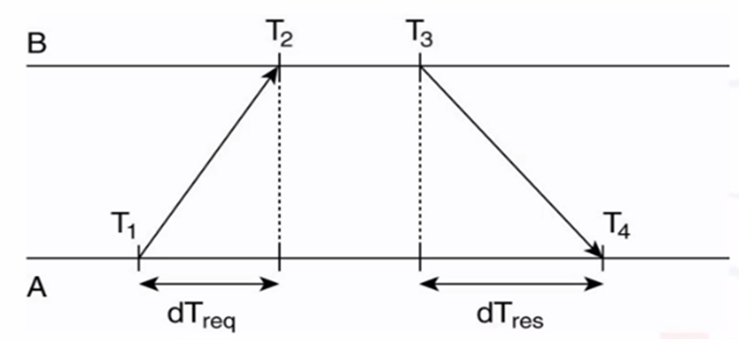
\includegraphics[width=80mm]{img/ntp.png}
    \end{figure}
    \bigbreak
    NTP è un protocollo di sincronizzazione client-server. Se non abbiamo GPS nel SD, ci resta di rivolgerci ad un server. C'è una gerarchia di server NTP (nel primo strato i server hanno orologi atomici, negli altri si introducono approssimazioni). 

    Il client A in T1 manda una richiesta ad un server NTP, il server riceve la richiesta al tempo T2, la processa e in T3 manda la risposta al client che la riceve in T4. Il problema è che c'è latenza tra client e server, se mi serve l'ora precisa devo tenerne conto (l'orologio sul client A non è preciso, se no non avrebbe motivo di chiedere l'ora, ma questo rende aleatorio parlare di un istante $T_x$). La soluzione è mettere i timestamp nei vari messaggi, il protocollo cerca di stimare il ritardo basandosi sui timestamp presenti nei messaggi scambiati, in questo modo cerca di aggiustare il tempo rendendolo più vicino a quello reale del time server. In NTP, il server è passivo perché risponde solamente a richiesta da parte di altri nodi ma non manda messaggi a nessuno di sua sponte.
    \bigbreak
    \textit{Il client NTP manda un time-request al server NTP. Come risultato di questo scambio, il client è in grado di calcolare il ritardo di collegamento e l'offset locale, ed è in grado di aggiustare il suo orologio locale in modo che sia uguale all'orologio del server}

    \item \textbf{The Berkeley Algorithm} 
    \bigbreak
    Questa soluzione si basa sul fatto che è sufficiente che i nodi in un sistema siano allineati tra loro senza che siano sincronizzati con il mondo esterno. Viene eletto uno dei nodi come coordinatore, time daemon. Il time daemon condivide il suo orario con tutti i nodi della rete, essi rispondono mandando la differenza tra i loro orari e quello del time daemon. Quest'ultimo calcola la media degli orari di tutti e comunica a tutti gli altri nodi di sincronizzarsi si questo orario comune. In realtà l'implementazione non è scontata: portare indietro un orologio è problematico (inconsistenza del file system).
    
    \begin{enumerate}
        \item Il time daemon è attivo perchè periodicamente manda un messaggio a tutti gli altri nodi (broadcast, arriva anche a sè stesso) ma non obbliga nessuno a sincronizzarsi
        \item Il nodo risponde con l'offset (differenza tra il proprio orologio e quello ricevuto), anche il time daemon risponde a se stesso con 0. Non manda UTC, manda il tempo del propprio orologio. 
        \item time daemon fa una media di tutti gli orologi presenti nella rete (utilizza questo tempo per sincronizzare tutti) e invia ad ogni nodo, compreso sé stesso, lo spostamento che devono effettuare per sincronizzarsi al tempo medio. 
    \end{enumerate}
\end{enumerate}    
\section{Sincronizzazione con orologio logico}
Il concetto di orologio logico è stato proposto da L.Lamport nel 1978, per gestire i casi in cui è necessario concordare la sequenza di eventi, senza doversi per forza sincronizzare gli orologi fisici. L'orologio logico di Lamport non è un orologio, è un contatore di eventi. \\ Dividiamo gli eventi in eventi interni (relativo al processing locale) ed eventi esterni (mandare/ricevere messaggi). 
\bigbreak
Ogni nodo ha un contatore inizializzato a zero che rappresenta il suo orologio logico. Ogni evento che succede incrementa il contatore (sia evento interno che esterno). Consideriamo un dato istante di tempo, gli orologi logici su nodi differenti possono avere differenti valori. 
\bigbreak
Lamport si basa sul concetto di ordinamento parziale e definisce una relazione happens-before: se a, b sono eventi - l'espressione $a \longrightarrow b$ denota una relazione "a accade prima di b". Se C(a) è il contatore assegnato al processo dove accade a, voglio che C(a) $<$ C(b).
\begin{figure}[h]
\centering
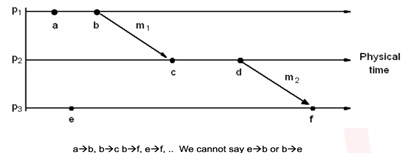
\includegraphics[width=90mm]{img/lamport.png}
\end{figure}
\bigbreak
Se a,b sono eventi sullo stesso terminale e l'evento a avviene prima dell'evento b, allora  $a \longrightarrow b$ vale. Se l'evento a è l'invio di un messaggio da parte di un processo e l'evento b è la ricezione dello stesso messaggio da parte del processo destinatario, allora  $a \longrightarrow b$ è vero. Se due eventi a, b avvengono in due processi diversi che non si scambiano messaggi, non posso dire nulla dell'ordine dei due eventi. 
\bigbreak
Se a è l'evento di mandare un messaggio $m$ da un nodo e b è l'evento di ricevere il messaggio su un altro nodo. Allora come assicuriamo, se  $a \longrightarrow b$, ad assicurare C(a) $<$ C(b)?
\begin{figure}[h]
\centering
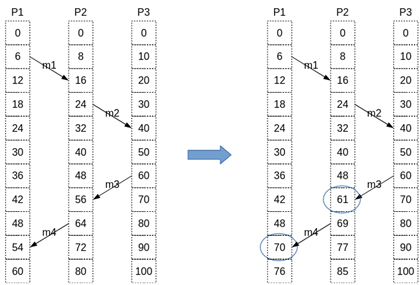
\includegraphics[width=90mm]{img/exla.png}
\end{figure}

\begin{enumerate}
    \item prima di eseguire un evento, il processo $P_i$ esegue $C_i \longrightarrow C_i + 1$
    \item quando il processo $P_i$ manda un messaggio \textit{m} a $P_i$ pone il timestamp di \textit{m} (Ts(m)) uguale a $C_i$ dopo aver eseguito lo step precedente
    \item quando $P_i$ riceve \textit{m}, aggiusta il suo contatore locale al valore $C_i = max\{C_i, Ts(m)\} + 1$
\end{enumerate}
Nell'esempio, a sinistra osserviamo che m1 e m2 sono giusti, in quanto il tempo di arrivo è superiore a quello di partenza del messaggio. Guardando m3 ci rendiamo conto del problema: il suo arrivo al tempo 56 non è compatibile con quello di partenza, che vale 60. Il processo P2 pone il suo orologio logico al valore 60+1. Analogamente m4 parte a 69, ma arriverebbe a 54. Al suo arrivo il processo P1 pone il suo orologio logico a 69+1. 
\bigbreak
\begin{figure}[h]
\centering
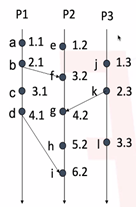
\includegraphics[width=30mm]{img/lamport2.png}
\end{figure}
\bigbreak
L'algoritmo può essere modificato. per ottenere un ordine totale, aggiungendo un ID di processo al timestamp dell'evento (un numero univoco che può essere assegnato ad ogni processo in un SD). \\ Il timestamp dell'evento e del processo $P_i$ viene $C_{i}(e).i$ dove .i è l'ID del processo. Mi serve in caso di pareggio: se ho lo stesso orario guardo informazione dell'ID e so chi va prima. \\ L'ordine totale di timestamp non significa che conosciamo la relazione temporale tra ogni coppia di eventi.
\bigbreak
\noindent \textbf{Multicasting con ordinamento totale} \\ Mettiamo caso che vi siano due client concorrenti A e B che vogliono caricare dei dati in due copie diverse in un DB replicato. Se usassimo Lamport in ordine parziale, non riusciremmo a caricare i dati nello stesso modo (nel DB1 arriverebbe prima la richiesta di A, nel DB2 quella di B), creando inconsistenza nei due DB. Per implementare il multicast con ordine totale c'è bisogno di assumere che non ci siano messaggi persi e che i messaggi dello stesso mittente vengano ricevuti nell'ordine in cui sono stati inviati.
\bigbreak 
Funzionamento:
\begin{enumerate}
    \item Il processo $P_i$ invia il messaggio $m_i$ munito di timestamp a tutti gli altri processi. Il messaggio viene messo in una coda locale i
    \item Qualsiasi messaggio in entrata di $P_j$ è accodato nella sua coda j in base al timestamp, e viene inviato un ACK di avvenuta consegna a tutti gli altri processi (gli eventi send e receive dei messaggi e ACK sono ordinati totalmente con Lamport)
    \item $P_j$ passa poi il messaggio $m_i$ all'applicazione sovrastante se: $m_i$ è in testa alla coda j e $m_i$ è stato ACKed, quindi ricevuto, da tutti gli altri processi
    \item Alla fine tutti i processi avranno quindi la stessa copia della coda locale, perciò tutti i messaggi sono passati all'applicazione nello stesso ordine in tutti i nodi. 
\end{enumerate}

\textit{Esercizio: ci sono due utenti e due DB di una banca che ospitano i conti correnti. Il primo utente versa 100euro sul conto e il secondo utente introduce l’interesse. A seconda dell’ordine di esecuzione delle operazioni sui DB mi cambiano i soldi che il primo utente ha in banca, il sistema bancario dev’essere consistente.
\bigbreak
Aiuti per esercizio: assumiamo che ci sia un processo per ciascun invidio di messaggio e due processi che curano l’aggiornamento dei DB (4 processi totali). Quando il messaggio è mandato viene mandato anche il timestamp. Il sistema funziona con gli ACK e code locali. Gli eventi di ricezioni, invio, ACK, sono ordinati con Lamport.}

\begin{figure}[h]
\centering
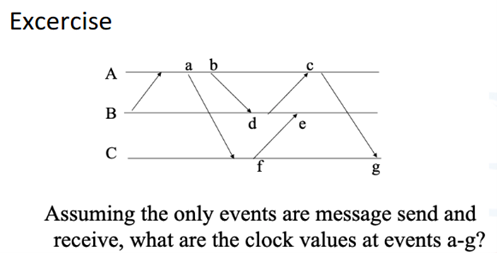
\includegraphics[width=100mm]{img/exla2.png}
\end{figure}

\section{Algoritmi di mutua esclusione}
Un insieme di processi deve accedere in modo concorrente a delle risorse condivise. Non condividendo la memoria, possono coordinarsi unicamente scambiandosi messaggi.
\bigbreak
\noindent Soluzioni in un sistema unico:
\begin{itemize}
    \item identificazione delle regioni critiche 
    \item uso di semafori o monitor per garantire che quando un processo è in regione critica nessuno altro possa entravi.
\end{itemize}
\bigbreak
\subsection{Algoritmo centralizzato} 
Scelgo un processo come coordinatore e l'accesso alla risorse è fatto in modalità client-server:
\begin{itemize}
    \item Il processo 1 chiede al coordinatore il permesso di entrare in sezioni critica, il permesso viene accordato
    \item Successivamente, il processo 2 chiede il permesso di entrare in regione critica. Il coordinatore non risponde ma inserisce 2 nella sua coda di attesa
    \item Quando il processo 1 esce dalla regione critica ed avvisa il coordinatore, il quale controlla nella sua coda e risponde affermativamente al primo processo presente, in questo caso il processo 2
\end{itemize}
L'algoritmo centralizzato comporta dei problemi: single-point-of-failure, meccanismo di timeout (se un nodo supera un tempo limite in cui tiene la risorsa, il coordinatore deve intervenire), collo di bottiglia del coordinatore nelle prestazioni ed è difficile distinguere l'inattività del coordinatore dall'indisponibilità della regione critica (il coordinatore non rispondendo non fa capire se è caduto o se mi ha messo in attesa).

\subsection{Algoritmo decentralizzato Ricart e Agrawala}
Devo assumere che ci sia un ordine totale degli eventi e un sistema di consegna di messaggi affidabile (ACK di TCP). 
\bigbreak 
\begin{enumerate}
    \item Se un processo P vuole usare una risorsa costruisce un messaggio e lo manda a tutti i processi (incluso sé stesso), il messaggio contiene:
    \begin{itemize}
        \item[-] nome della risorsa (potrebbero essercene più di una)
        \item[-] ID del processo
        \item[-] timestamp corrente (non fisico, Lamport)
    \end{itemize}
    \item Quando un processo Q riceve un messaggio si distinguono 3 casi:
    \begin{enumerate}
        \item Se Q non è in RC e non vuole entrarci risponde con un OK a P
        \item Se Q è in RC non risponde e accoda la richiesta (P deve riceve OK da tutti i nodi per entrare in RC)
        \item Se Q vuole entrare in RC ma non l'ha ancora fatto, confronta il timestamp del messaggio con quello del messaggio che lui ha mandato a tutti gli altri. Il minore vince. Se quello inviato da P è il minore risponde OK a P, altrimenti accoda il messaggio ad entra in RC.
    \end{enumerate}
    \item Il processo P dopo aver inviato il messaggio aspetta l'OK da tutti per poi entrare in RC
    \item Quando P esce da RC manda un messaggio di OK a tutti i processi nella propria coda di attesa, svuotandola
\end{enumerate}

\begin{figure}[h]
\centering
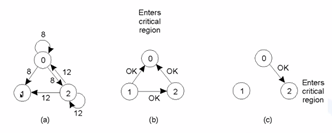
\includegraphics[width=90mm]{img/ricart.png}
\end{figure}
Il processo 0 e il processo 2 vogliono la stessa risorsa nello stesso momento e costruiscono i messaggi. P0 manda a tutti un messaggio con timestamp = 8 mentre P2 manda un messaggio con timestamp = 12. P1 manda un OK ad entrambi, P0 e P2 sanno che vogliono accedere alla stessa risorsa, ma P2 vede che il suo timestamp è maggiore e lascia entrare P0, mandandogli l'OK. P0 confronta i timestamp, vede di avere il minore e accoda P2, aspettando l'OK da tutti i processi.  Una volta che P0 ha finito manda un OK a tutti gli altri nodi che ha in coda che hanno richiesto la risorsa. 
\bigbreak
\noindent Problemi:
\begin{itemize}
    \item Non c'è risposta da un processo perché crasha, blocco tutto
    \item Comprendere tutti i nodi della rete può essere uno spreco di risorse
\end{itemize}

\subsection{Algoritmo dell'anello}
C'è un layer di overlay: considero un gruppo di processi non necessariamente ordinato (supponiamo di poter dare un ID univoco a ciascun processo in esecuzione) e costruisco un anello logico. Questo modello è stato usato nei primi modelli di rete LAN, il modella era chiamato token-ring
\bigbreak
Immaginiamo che sia un token unico, l'idea è che chi lo possieda possa accedere alla risorsa condivisa. Inizialmente il token viene assegnato ad un processo, se il processo è interessato entra nella regione critica e solo quando vi esce passa il token. Il token è mandato - tramite un messaggio - dal processo \textit{i} al processo \textit{(i+1)mod n}. Se il processo è interessato alla risorsa, può accedervi quando riceve il token. Per questi fairness lo stesso token non può essere usato per accedere due volte alla stessa risorsa. 
\bigbreak
\noindent Problemi:
\begin{itemize}
    \item un processo smette di funzionare, se i processi hanno l'indirizzo solo del successivo processo nell'anello, l'anello si romperà (risolviamo memorizzando k indirizzi) 
    \item se si ferma il processo che tiene il token, il token va perso
\end{itemize}

\subsection{Confronto tra i 3 algoritmi }
\begin{figure}[h]
\centering
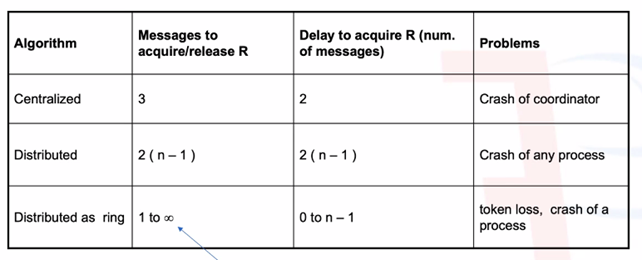
\includegraphics[width=110mm]{img/confronto.png}
\end{figure}
 L'approccio centralizzato richiede un minore numero di di messaggi (se un processo deve entrare in RC si scambia tre messaggi con il server). Nel distribuito è maggiore perché c'è una sorta di broadcasting tra tutti i nodi. Nell'approccio ad anello è infinito perché il token potrebbe girare all'infinito senza che nessuno lo prenda (se nel sistema c'è una risorsa che viene usata raramente, il token ring non è comodo).
 \bigbreak
 L'approccio centralizzato ha un ritardo nell'acquisizione della risorsa = 2, faccio la richiesta al server e il server mi risponde. Nell'anello teoricamente devo aspettare il token, se lo possiedo il mio ritardo è 0, se l'ho appena lasciato devo aspettare n-1. Suppongo che nel distribuito sia 2(n-1) in quanto devo mandare un messaggio a tutti gli altri n-1 nodi per chiederli se posso entrare in RC, in più devo aspettare l'OK di tutti i nodi per poterci entrare. 

\section{Algoritmi di elezione}
Eleggere un coordinatore può essere utile (ex. implementare una soluzione centralizzata per mutua esclusione). Gli algoritmi di elezione tipicamente puntano ad eleggere il processo attivo con l'ID maggiore (i processi si distinguono per un ID univoco, come indirizzo di rete + numero del processo. Non c'è perdita di generalità: potrei scegliere il processo con carico di lavoro più basso impostando $ID(P_i) =< 1/load(P_i)$). In alcuni algoritmi di suppone che tutti i processi conoscano l'ID degli altri (non sanno comunque se i processi sono attivi o meno). 

\subsection{Algoritmo del bullo}
\begin{figure}[h]
\centering
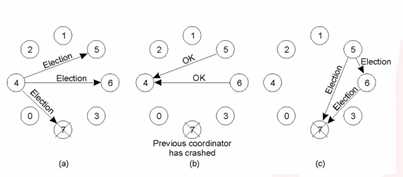
\includegraphics[width=90mm]{img/bullo.png}
\end{figure}
\begin{enumerate}
    \item[-] Figura a) Il processo 4 si accorge che non c'è un coordinatore (scade un timeout). Capisce che dev'essere indetta un'elezione ma non lo comunica a tutti i processi della rete, lo comunica solo ai processi con ID maggiori del suo. 
    \item[-] Figura b) il processo 5 e 6 sono attivi e con ID più alto, l'algoritmo dice che debba essere mandato un OK quando si riceve un messaggio di elezione da un processo con ID minore, mandano OK al processo 4. Il processo 7 non è attivo e non risponde. 
    \item[-] Al processo 4 basta riceve un solo OK da un processo con ID più alto del suo per sapere che non sarà lui il coordinatore
    \item[-] Figura c) I processi 5 e 6 mandando un messaggio di elezione a processi con ID maggiori del loro
    \item[-] Il processo 6 a questo punto manderà OK al processo 5, il processo 5 sa che non sarà lui il coordinatore
    \item[-] Il processo 6 ha mandato un messaggio anche al processo 7, il quale non è attivo. Dopo un certo tempo, scade un timeout nell'orologio del processo 6: il processo 6 capisce di essere lui il coordinatore.
    \item[-] Il processo 6 manda in broadcast il fatto di essere lui il nuovo coordinatore
\end{enumerate}

\subsection{Algoritmo di elezione ring-based}
Assunzioni:
\begin{itemize}
    \item I processi sono logicamente ordinati come un anello: il processo $P_k$ ha un canale di comunicazione con $P_{k+1}modn$
    \item I messaggi circolano in senso orario senza fallimenti
    \item Ogni processo ha un ID unico
\end{itemize}
Obbiettivo: eleggere il processo attivo con ID maggiore. Dev'essere unico anche nel caso vengano indette più elezioni
\begin{figure}[h]
\centering
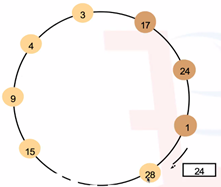
\includegraphics[width=65mm]{img/elering.png}
\end{figure}
\begin{enumerate}
    \item Tutti i processi sono marcati come non partecipanti (variabile booleana). Questo serve per fermare il prima possibile messaggi di elezioni diverse che potrebbe portare ad esiti diversi
    \item Quando un processo $P_k$ capisce che il coordinatore non sta rispondendo indice un'elezione marcando sé stesso come partecipante e mandando al nodo successivo nell'anello un messaggio di elezione con il proprio ID: \\ $<ELECTION, ID(P_k)>$
    \item Quando un processo $P_m$ riceve un messaggio di elezione da $P_k$, se:
    \begin{itemize}
        \item [-] se ID($P_k$) $>$ ID($P_m$) \\ $P_m$ marca sé stesso come partecipante e fa proseguire il messaggio nell'anello 
        \item [-] se ID($P_k$) $<$ ID($P_m$) \\ se $P_m$ è non partecipante, cambia il suo stato e invia il messaggio \\ $<ELECTION, ID(P_m)$. \\ Se $P_m$ è marcato come partecipante, non inoltra il messaggio perché capisce che non c'è nessun altro processo con un ID maggiore del proprio)
        \item [-] se $k = m$ \\ l'ID ricevuto è il proprio allora si è il coordinatore: marca sé stesso come non partecipante e invia il messaggio $<ELECTION, ID(P_m)$ ai nodi successivi
    \end{itemize}
    \item Quando un processo $P_k$ riceve il messaggio $<ELECTION, ID(P_m)$, marca sé stesso come non partecipante, salva l'ID del coordinatore 
\end{enumerate}
\noindent \textbf{Gestione dei guasti}: i guasti dovuti al crash di uno dei nodi nell'anello vengono gestiti da ciascun processo memorizzando, non solo l'indirizzo del processo successivo, ma anche alcuni altri che lo seguono nell'anello. Se la comunicazione con il processo successivo fallisce, il messaggio viene inviato al primo attivo tra quelli che lo seguono
\bigbreak
\noindent \textbf{Elezioni concorrenti}: l'uso dello stato partecipante/non partecipante aiuta a spegnere il prima possibile i messaggi non necessari in elezioni simultanee. Se un messaggio di elezione arriva ad un nodo già partecipante, non viene più inoltrato
\bigbreak
\noindent \textbf{Caso peggiore}: nel caso peggiore questo algoritmo necessita di 3(n-1) messaggi per eleggere un coordinatore. Ho il caso peggiore quando l'assenza del coordinatore è notata dal processo con ID minore (cioè il nodo più vicino in senso antiorario al coordinatore). In questo caso abbiamo bisogno di n-1 messaggi per raggiungere il nodo con ID maggiore, altri n messaggi per concludere l'elezione e n per annunciare il coordinatore. 

\begin{figure}[h]
\centering
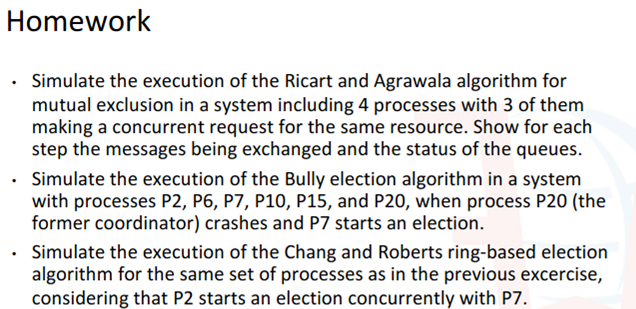
\includegraphics[width=100mm]{img/compitielezione.png}
\end{figure}

\chapter{Fault tolerance e consenso}
La fault tolerance ci permette di valutare la qualità di un SD: ovviamente maggiore è il numero di nodi partecipanti - e quindi il numero di connessioni di rete coinvolte - e più alta è la probabilità che uno dei nodi o uno dei collegamenti possa presentare un malfunzionamento in termine di ritardi dei messaggi, crash dei processi e nodi compromessi (malevoli). Questi malfunzionamenti vengono anche individuati come partial failure. 
\bigbreak
Lo scopo di un SD è fornire trasparenza rispetto ai guasti, cioè ovviare al malfunzionamenti senza che l'utente se ne accorga
\bigbreak
Essere resistente ai guasti è fortemente correlato a quelli che vengono chiamati sistemi affidabili (dependable systems). I sistemi affidabili che offrono dependability, implicano:
\begin{itemize}
    \item Availability - Disponibilità: probabilità che il sistema funzioni correttamente in ogni singolo momento. Un sistema ad alta disponibilità può essere molto affidabile per reboot giornalieri
    \item Reliability - Affidabilità: abilità di funzionare correttamente per un lungo periodo di tempo. Un sistema con alta reliability può non avere alta availability: uptime di 11 mesi ma down per un mese per manutenzione
    \item Safety - non è sicurezza: un fallimento parziale non deve portare al fallimento totale del sistema
    \item Maintainability: capacità e facilità di riparare il sistema
\end{itemize}
\newpage
\noindent Ci sono vari tipi di malfunzionamento possibili
\begin{figure}[h]
\centering
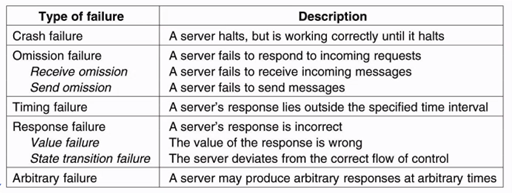
\includegraphics[width=110mm]{img/fault.png}
\end{figure}

\section{Mascheramento dei guasti con ridondanza}
Ci sono varie tipologie di ridondanza:
\begin{enumerate}
    \item Ridondanza di informazioni: extra bit sono aggiunti per correggere e ricostruire gli errori dovuti al rumore sul canale
    \item Ridondanza temporale: il malfunzionamento potrebbe essere temporaneo. Riprovo a fare la stessa operazione: ripeto una transazione ad esempio. Per le RPC questo richiede un ulteriore livello di attenzione: se sono idempotenti, possiamo farlo (come la open()).
    \item Ridondanza fisica: extra HW o SW (processi) vengono aggiunti per ripristinare un fallimento di una componente. Ex. RAID di HDD.
\end{enumerate}

\begin{figure}[h]
\centering
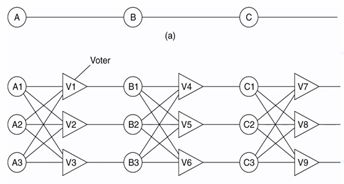
\includegraphics[width=90mm]{img/ridondanza.png}
\end{figure}
\noindent Figura a) C'è un circuito di 3 nodi che si passano informazioni. Se uno di loro funziona male, c'è un alta probabilità che questo circuito sia errato. \\ Figura b) vediamo un esempio di failure masking su tre nodi che si scambiano informazioni (da A a B, da B a C) usando ridondanza. \\ Prendo tre copie del nodo A e metto dei \textbf{voter} che ricevono in ingresso l'output di tutte le copie di A, e ridanno in uscita la maggioranza tra questi output (A1 e A2 dicono 10, A3 dice 5: il voter prende 10). Se non c'è maggioranza manda in uscita "unknown". Ne consegue che per ogni nodo debbano funzionare almeno due nodi replica, sono resistente al fallimento di un nodo replica. 
\bigbreak
Ne segue che: un sistema si dice \textbf{k-fault tolerance} se continua a funzionare correttamente anche se k componenti smettono di funzionare

\subsection{Resilienza e ridondanza nei processi}
La ridondanza può essere applicata anche ai processi. Posso creare un gruppo di processi identici che usano lo stesso dato. Ogni processo riceve i messaggi del gruppo. \\ Quanta ridondanza è necessaria? Quanti processi metto in un gruppo?
\begin{itemize}
    \item Crash failure: sono sufficienti k+1 processi per fornire k-fault tolerance (i client ottengono lo stesso valore dai processi sopravvissuti)
    \item Responde failure (valori errati ridati dai processi): in questo caso sono sufficienti 2k+1 processi per k-fault tolerance (il client può decidere votando)
    \item Se c'è bisogno di consenso nel gruppo (mutua esclusione, elezione) la cosa è più complicata. Servono, in una situazione senza nodi malevoli, 3k+1 processi. In alcuni casi ciò è impossibile, in particolare quando la maggioranza dei nodi sono malevoli. 
\end{itemize}

\section{Problemi di consenso}
I processi in un gruppo devono mettersi d'accordo su chi di loro ha ragione. Ci sono algoritmi per deciderlo ma funzionano sotto determinate condizioni. 
\bigbreak
Problemi di consenso:
\begin{itemize}
    \item [-] Consenso: ogni processo propone un valore unico e i processi non difettosi dovrebbero concordare sullo stesso valore. Gli algoritmi di consenso hanno l'obbiettivo di fare in modo che un insieme di nodi concordino riguardo allo stato complessivo del sistema in ogni istante di tempo 
    
    (ad ex. Facebook è distribuito su molti nodi di calcolo distribuiti per il mondo, ciascuna utente si collega e vorrebbe trovare la stessa visione dell'homepage, dell'elenco dei propri amici indipendentemente da quale macchina gli risponde).
    
    \item [-] Problema dei generali bizantini: un processo (comandante) propone un valore v. Tutti i processi corretti devono concordare su un valore. Se il comandante non è difettoso, concordano su v.
    
    (ad ex. A differenza di FB, in Bitcoin i nodi possono comportarsi in modo malevolevo ed eseguire il protocollo in modo volutamente errato al fine di violare la coerenza del sistema a proprio vantaggio (double spending). Questo tipo di comportamento viene detto bizantino e l'algoritmo di consenso deve fare in modo che i nodi onesti non vengano influenzati dai nodi malevoli, in modo da raggiungere uno stato consistente)
    
    \item[-] Consistenza interattiva: ogni processo propone un valore. Tutti i processi non-faulty concordano su un vettore di valori composto filtrando valori proposti
\end{itemize}
\noindent La soluzione dipende da diversi fattori:
\begin{itemize}
    \item Il sistema è sincrono o asincrono?
    \item Il delay della comunicazione è legato a qualche proprietà o è arbitrario?
    \item L'invio dei messaggi è ordinato (prima 1 poi 2) o no?
    \item La trasmissione dei messaggi avviene in unicast o multicast?
\end{itemize}
\bigbreak
\noindent \textbf{Esempio sul consenso dei generali bizantini} 
\bigbreak
\begin{figure}[h]
     \centering
     \begin{subfigure}[b]{0.3\textwidth}
         \centering
         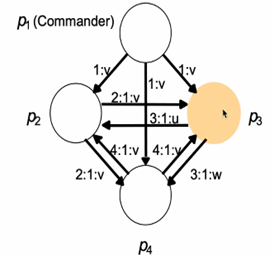
\includegraphics[width=50mm]{img/biz1.png}
     \end{subfigure}
     \hfill
     \begin{subfigure}[b]{0.5\textwidth}
         \centering
          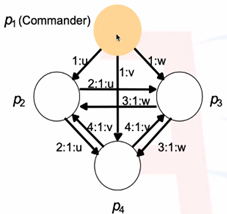
\includegraphics[width=50mm]{img/biz2.png}
     \end{subfigure}
\end{figure}
\noindent Ho N = 4 processi, di cui K = 1 sono di tipo "bizantino". Ci sono delle assunzioni fatte da Lamport: processi sincroni, comunicazione unicast, delay limitato, ordine dei messaggi preservato. \\ Ogni processo produce un valore $V_i$. Gli $N-K$ nodi funzionanti devono sapere come accordarsi su un vettore corretti di valori, isolando i dati errati. \\ In questo caso per far sì che ci sia consenso, servono almeno 3k+1 processi funzionanti. 
\bigbreak
\noindent Funzionamento: 
\begin{enumerate}
    \item Il comandante invia un valore a ciascuno dei luogotenenti
    \item Ciascun luogotenente inoltra il valore ricevuto ai suoi pari (sono necessari più round per N$>$4)
    \item Un luogotenente riceve un valore del comandante, più N-2 valori dai suoi pari:
    \begin{itemize}
        \item [-] se il comandante è difettoso, tutti i luogotenenti non sono difettosi e ognuno avrà raccolto esattamente l'insieme di valori che il comandante ha inviato
        \item[-]  se uno dei luogotenenti è difettoso: ciascuno dei suoi pari corretti riceve N-2 copie del valore inviato dal comandante, più un valore inviatogli dal luogotenente difettoso
        \item[-] In entrambi i casi, i luogotenenti corretti devono solo applicare una funzione di maggioranza semplice all'insieme di valori che ricevono
        \item[-] Quando no esiste una maggioranza, viene usato un valore speciale
    \end{itemize}
\end{enumerate}
\noindent \textbf{Il consenso bizantino necessita di almeno 3k+1 processi, dove k sono processi faulty}

\section{Consenso in sistemi asincroni/sincroni}

Sistemi sincroni:
\begin{itemize}
    \item[-] L'esecuzione su ogni nodo è limitata in termini di velocità e tempo
    \item[-] I collegamenti di comunicazione hanno un ritardo di trasmissione limitato
    \item[-] L'orologio su ogni nodo ha una deriva limitata
\end{itemize}
\noindent Sistemi asincroni:
\begin{itemize}
    \item[-] L'esecuzione su ogni nodo avviene a velocità arbitraria
    \item[-] I collegamenti di comunicazione hanno un ritardo di trasmissione diverso e illimitato
    \item[-] L'orologio su ogni nodo ha una deriva, drift, illimitata
\end{itemize}
\newpage
\noindent Possiamo fare delle osservazioni:
\begin{itemize}
    \item I sistemi distribuiti eterogenei basati su Internet sono intrinsecamente asincroni
    \item Il coordinamento e l'accordo nei sistemi asincroni sono difficili e spesso impossibili. Facciamo spesso ipotesi (parziali) sulla sincronicità
    \item Per cooperare al raggiungimento di un obbiettivo comune abbiamo bisogno di algoritmo che raggiungano una forma di sincronizzazione
\end{itemize}

\subsection{Impossibilità di accordo in sistemi asincroni}
\noindent \textbf{Teorema FLP (1985)}: E' impossibile risolvere il problema di consenso in sistema asincroni: quando i ritardi nella risposta ai messaggi sono arbitrari non esiste una soluzione garantita all'accordo bizantino (consenso in presenza di fallimenti bizantini) né al multicast totalmente ordinato, anche se un nodo singolo fallisce. \\  Altrimenti detto: in un SD asincrono in cui sono possibili fallimenti, non è possibile avere un protocollo deterministico per raggiungere il consenso. \\ Esistono soluzioni per sistemi parzialmente sincroni che possono essere utilizzati per modella sistemi reali. 
\bigbreak
\noindent \textbf{Teorema CAP}: negli storage r/w, non posso avere le seguenti proprietà tutte insieme:
\begin{enumerate}
    \item Consistency (Consistenza): ogni lettura la scrittura più recente o un errore (implica comunque che tutti i nodi vedano gli stessi dati)
    \item Availability (Disponibilità): ogni richiesta riceve una risposta (il sistema è operativo in un dato momento)
    \item Partition Tolerance: il sistema tollera un numero arbitrario di messaggi persi (o ritardi)
\end{enumerate}
I sistemi reali non vogliono solitamente rinunciare al Partition Tolerance, per cui hanno un approccio rilassato verso Disponibilità e Consistenza. 
\begin{figure}[h]
\centering
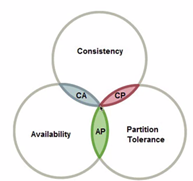
\includegraphics[width=50mm]{img/cap.png}
\end{figure}

\section{Consenso in pratica}
La correttezza in un algoritmo distribuito è espressa tramite la \textit{safety} e la \textit{liveness}. La prima dice che non succederà mai nulla di brutto: il processo non entrerà mai in uno stato inaccettabile (non sarà possibile dimostrare in un momento successivo che la decisione corretta era un'altra). La seconda ci dice che eventualmente accadrà qualcosa di bello, cioè il processo entrerà in uno stato che ci garba (il protocollo consente sempre di raggiungere una decisione, corretta o sbagliata che sia).
\subsection{Protocollo Paxos}
Introdotto da Lamport nel 1989, ne esistono molte versioni, ha come obbiettivo il consenso in una rete di processi inaffidabili. 

Paxos è un protocollo per raggiungere il consenso in SD: è safe ma non live e non tollera nodi bizantini nella sua versione base. Paxos serve a raggiungere consenso su un valore, i nodi che partecipano possono avere ruoli diversi e l'esecuzione è divisa in turno. 
\bigbreak
\noindent Ruoli dei processi:
\begin{itemize}
    \item Proposer: sceglie un valore da votare e lo propone a tutti
    \item Acceptor: riceve la proposta dal proposer, la voto o meno
    \item Learner: memorizza il valore votato dalla maggioranza
\end{itemize}
\noindent Esecuzione del protocollo:
\begin{enumerate}
    \item Un proposer avvia un turno di votazione, inviando a tutti un messaggio che chiamiamo \textit{prepare}
    \item Gli acceptor che lo ricevono, possono rispondere con una \textit{promise}, impegnandosi quindi a votare quel turno
    \item Il proposer sceglie un valore e lo manda a tutti con un \textit{accept}
    \item Gli acceptor dicono ai learner di imparare quel valore con un \textit{learn}
\end{enumerate}
\begin{figure}[h]
\centering
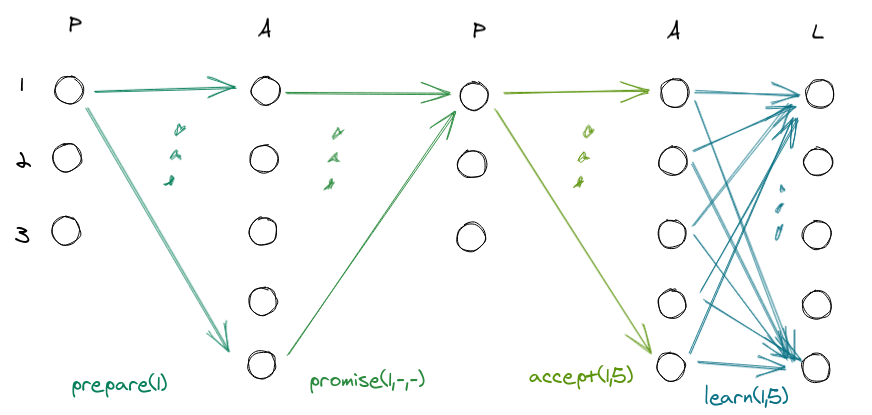
\includegraphics[width=110mm]{img/paxos.png}
\end{figure}
\bigbreak
\noindent In immagine:
\begin{itemize}
    \item [-] P, A, L sono Proposer, Acceptor, Learner
    \item [-] Abbiamo 3 proposer, 5 acceptor e 5 learner
    \item [-] Il grafico è temporale e le frecce rappresentano i messaggi scambiati tra i nodi
    \item [-] Ogni proposer ha un turno associato (proposer 1 - turno 1, proposer 2 - turno 2, proposer 3 - turno 3)
\end{itemize}
\noindent Cosa succede:
\begin{enumerate}
    \item Il proposer 1 inizia il protocollo e manda a tutti un prepare(1) in cui specifica il turno
    \item Gli acceptor rispondono con una promise (1, -, -) che contiene il turno, ultimo turno a cui ha partecipato (nessuno per ora) e ultimo valore votato (nessuno per ora). Gli acceptor si impegnano anche a non partecipare a eventuali turni più vecchi di quello del proposer. 
    \item Il propose se riceve più della meta delle promise, e può quindi inviare a tutti un accept(1,5), specificando il valore (5) da votare per il turno (1). \item Gli acceptor votano inviando al learner la loro intenzione con learn(1,5), valore e il round. 
\end{enumerate}
A questo punto la votazione del primo proposer è andata, inizia un nuovo turno il secondo proposer: 
\begin{enumerate}
    \item Il proposer 2 avvia un nuovo turno con r = 2
    \item Gli acceptor ricevono prepare(2) e decidono di prendere parte a quel turno, quindi rispondono con una promise(2, 1, 5), cioè indicano di prendere parte al turno 2, e informano che l'ultima volta che hanno votato era per il turno 1 ed hanno votato 5.
    \item Il proposer riceve almeno la metà delle risposte e propone un valore, che deve per forza essere 5
    \item Gli acceptor ricevono la risposta e mandano il learn al learner. 
\end{enumerate}
Il proposer deve per forza scegliere 5 perché Paxos è un protocollo per raggiungere consenso. Il secondo proposer si rende conto che il valore di consenso è stato scelto nel turno precedente, ed è 5. 
\bigbreak
\noindent \textbf{Safety}: qualunque scelta venga fatta dal protocollo è corretta, non è possibile che in un turno r'$>$ r si scopra che il valore di consenso scelto nel turno r sia sbagliato.
\noindent \textbf{Liveness}: ci sono dei casi in cui il protocollo non compie una scelta. La chiave è proprio nel significato di promise(r, lr, lv), in cui l'acceptor promette al proposer di votare per il turno r e di ignorare tutti i messaggi relativi a turni r' $<$ r. \\ Paxos tollera k nodi faulty con N = 2k+1

\subsection{Protocollo Raft}
Ogni nodo si può trovare in tre stati: follower, candidate, leader. \\ Tutti i nodi partono nello stato di follower, se un nodo follower non sente che c'è un leader (scade un timeout) passa allo stato di candidate. Il nodo candidato manda una richiesta di voto verso tutti gli altri nodi e gli altri nodi rispondono con il loro voto. Il nodo candidate diventa leader se ottiene voti dalla maggioranza dei nodi del sistema. Tutti i cambiamenti apportati al sistema passando dal leader da ora in avanti. Ogni cambiamento è aggiunto come entry nel log del leader, i leader inoltra questo cambiamento a tutti i nodi follower e aspetta che la maggioranza dei nodi abbiamo scritto la nuova entry. A questo punto lo stato del nodo leader cambia e dice ai nodi follower che la entry è stata settata. 

\chapter{Distributed Ledger Technologies (DLT) e Blockchain}
DLT è un registro distribuito avente moltissime applicazioni. Un esempio di DLT è Blockchain (2008), creata dal paper "Bitcoin: A peer to peer electronic cash system" di Nakamoto". Blockchain è una tecnologia usata non solo per Bitcoin, essa implementa un registro delle attività che avvengono (registro delle transazioni immobiliare del catasto è centralizzato, ma potrei farlo con blockchain). 
\bigbreak
\noindent \textbf{Sistema DLT} \\
E' un sistema distribuito con:
\begin{itemize}
    \item controllo decentralizzato
    \item i nodi sono gestiti da entità differenti e non si fidano uno dell'altro (comportamento bizantino)
    \item una copia di record di dati è memorizzata su ogni nodo
\end{itemize}
Nasce un problema di consenso: questi nodi devono essere d'accordo sull'intera storia dei dati. 

\section{Blockchain}
E' una sequenza storica di transazioni, di record di dati (Alice trasferisce 0.15BTC a Bob). 
\bigbreak

Ogni transazione è firmata digitalmente (in BC si utilizza il meccanismo a chiave asimmetrico, ogni nodo ha una chiave pubblica e una privata. La transazione si firma con la chiave privata) e propagata a tutti i nodi partecipanti. Quando un nodo riceve una transazione, deve validarla: validare una transazione è dipendente dall'applicativo, in un contesto finanziario il nodo potrebbe controllare la propria storia e vedere se il mittente abbia ricevuto soldi e quindi se ne abbia abbastanza per la transazione che sta provando a fare (le transazioni validate sono ancora "pending" perché non fanno ancora parte della catena). 
\bigbreak
\noindent \textbf{Cos'è un blocco?}
Le transazioni pending (ne arrivano molte e si accumulano) si raggruppano in un blocco (blocchi con numero variabile di transazioni) che ha un timestamp (non di ciascuna transazione, appartiene al blocco). 
\begin{figure}[h]
\centering
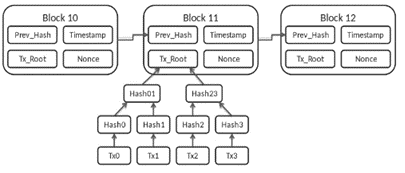
\includegraphics[width=90mm]{img/block.png}
\end{figure}
In figura vediamo cosa c'è dentro i blocchi:
\begin{itemize}
    \item TxRoot: struttura dati (Merkel tree) per memorizzare le transazioni che appartengono al blocco, in questo esempio ci sono 4 transazione ($T_{x0}, T_{x1}, T_{x2}, T_{x3}$. Il Merkel tree rende molto efficiente sapere se una transazione è contenuta nel blocco guardando le funzioni di hash della radice
    \item PrevHash: è una catena quindi ho bisogno di collegare un blocco all'altro. Calcolo una fingerpint digitale del blocco precedente e lo scrivo nel blocco successivo
    \item Nonce: numero da cambiare per cercare di validare il blocco
\end{itemize}
Ogni nodo ha una copia di tutta la catena di blocchi, ma ogni nodo non ha un tempo diverso? I blocchi e le transazioni potrebbero avere timestamp diversi a seconda del nodo perchè non esiste la sincronizzazione precisa dei clock. Devo avere un sistema che mi garantisca la sincronizzazione del timestamp entro un'approssimazione.
\bigbreak
\noindent \textbf{Problemi} \\
I sistemi di cui parliamo sono asincroni, molto difficili da gestire. Abbiamo latenza non prevedibile, sincronizzazione impresa degli orologi e nodi che potrebbero essere malevoli (bizantini) quindi:
\begin{itemize}
    \item [-] L'ordine di arrivo delle transazioni può essere diverso per ciascun nodo (la propagazione del portafoglio di Alice non è istantanea per tutti, ritardi di rete)
    \item [-] Alcune transazioni potrebbero contraddirsi a vicenda (Alice vuole fare la furba e spende 0.2BTC in due negozi diversi cercando di sfruttare i ritardi di propagazione)
    \item [-] Nodi diversi potrebbero costruire differenti blocchi (nodi potrebbero avere transazioni diverse e quando creano il blocco lo fanno mettendoci dentro transazioni differenti)
    \item[-] Nodi diversi potrebbero avere, alla fine, catene diverse e quindi nessun consenso. 
\end{itemize}

\subsection{Consenso nella blockchain}
Il goal è far concordare i nodi sui blocchi e sulla sequenza di blocchi. 
\bigbreak
Viene calcolata l'hash function di ciascuna transazione e di un blocco. Quando calcolo l'hash del blocco inserisco negli input anche l'hash del blocco precedente nella catena e ci metto dentro anche un trucchetto Proof of Work. Il PoW rende la computazione dell'hash del blocco molto dispendiosa ma facile da verificare. Alcuni nodi volontari della catena, miner, cercano di calcolare l'hash del blocco, alla fine di questo lavoro è quasi immediato verificare se la computazione dell'hash sia stata eseguita correttamente o meno. Se ho molti nodi volontari, essi competono sul blocco, il vincitore è il nodo che risolve prima l'enigma brute-forcing. 
\bigbreak
La risoluzione del calcolo di un hash per un blocco riguarda il trovare un valore per \textbf{nonce} tale per cui il valore dell'output dell'hash sia minore di un certo numero (l'hash del blocco è una stringa alfanumerica, per sapere se è minore di un certo numero guardo quanti zeri ci sono a sx della stringa).
\bigbreak
La BC non è altro che una sequenza di blocchi: ogni blocco oltre a specificare il campo nonce, prende in input - per calcolare l'hash - l'hash calcolata per il blocco precedente. Se modifico qualche campo di input di un blocco, ne modifico l'hash finale e l'intera catena successiva non sarà più valida (se modifico un valore in input, il nonce trovato dai miner non mi restituirà più un hash con \textit{n} zeri davanti. Per risolvere dovrei ri-minare a partire da quel blocco fino al blocco più recente nella catena. Decisamente impegnativo da fare.
\bigbreak
Quando un miner risolve il problema matematico lo annuncia a tutti gli altri nodi della rete e manda a tutti i nodi il blocco e l'hash che dimostra che ha risolto il problema (è facile verificare se è corretto o meno), il blocco verificato viene aggiunto alla copia locale della catena. 
\bigbreak
Il lavoro dei miner è reso sempre più complesso al crescere della bravura e del numero di essi. Uso un problema matematico che si risolve con la brute forcing, che può aumentare di complessità nel tempo e che può avere alta varianza (risolvibile subito o tra anni) in modo da evitare che ci siano più vincitori in contemporanea. 
\bigbreak
In generale, ci dev'essere consenso tra tutti i nodi, cioè devono avere la stessa catena per tutti. Devo avere almeno la maggioranza dei nodi che non hanno un comportamento bizantino, dovrei riuscire a fare un attacco che è fatto dalla maggioranza dei nodi. 
\bigbreak
La catena può avere dei branch, siamo in una modalità concorrente (i processi vengono eseguiti su nodi diversi e non è possibile prevedere chi finisce prima o dopo, per cui è possibile che arrivano due blocchi, che contengono un'intersezione di transazioni, entrambi minati e validati). Siccome entrambi i blocchi hanno un puntatore al blocco precedente, è possibile che vengano a creati delle diramazioni nella catena. L'algoritmo fa in modo che ci sia una catena che si sviluppa più velocemente delle altre, i branch dopo un po' non vengono più sviluppati e si fermano. Se il miner capisce che il suo blocco non è parte della catena prevalente, il pool di transazioni che non fanno parte di un blocco già validato, viene rimesso nelle transazioni pending. 
\bigbreak
BC non memorizza il saldo di ogni utente, per sapere quanti soldi ha un utente nel portafoglio, devo scorrere a ritroso la catena e ricostruirlo (se devo pagare qualcosa, il sistema guarda indietro e vede se ce una transazione che garantisce che questi soldi ci siano). 

\subsection{Proprietà e limiti di blockchain}
\begin{itemize}
    \item Assumendo che la maggior parte dei nodi lavorano su una stessa catena, questa catena che cresce più velocemente sarà la più lunga e quella di cui ci fideremo
    \item Per fare in modo che un nodo malevolo possa cambiare una transazione in un blocco intermedio, deve ricalcolare tutte le funzioni di hash (trovando il valore di nonce) dei blocchi successivi e prevalere su tutti i nodi della rete
    \item BC è sicura fino a che il 50\% dei nodi miner è onesto
    \item BC non è necessariamente Proof of Work, può essere usata con algoritmo diversi (guardare Proof of Stake)
\end{itemize}
BC comporta anche dei problemi:
\begin{itemize}
    \item BTC consuma molto: viene comprato HW specializzato - non usabile per molto altro - che dev'essere poi smaltito e consuma molta elettricità (più di Google, come l'Olanda)
    \item In ambito finanziario vorremo eseguire transazioni ad alta frequenza, BTC permette poche transazioni a causa della fase di validazione
\end{itemize}

 \noindent \textbf{Permissionless DL}: tutti i nodi sono alla pari e svolgono lo stesso lavoro,l'accesso al registro delle transazioni è senza condizioni, le transazioni sono immutabili e vengono validate dai nodi stessi e vi e un principio di pseudo-anonimato tra i partecipanti. Bitcoin e Ethereum sono così, chiunque può partecipare alla rete come nodo o come miner e avere un wallet. I partecipanti sono pseudo-anonimi, vengono identificati da una chiave pubblica e non da nome e cognome.
\bigbreak

\noindent \textbf{Permissioned DL}: è un DL decentralizzato che tratta tutte le transazioni, fatta da uno o più sistemi di terze parti dato (ad es. una banca). Per entrare all'interno della chain si ha bisogno di un consenso, ciò vuol dire che i nodi non svolgono tutti lo stesso ruolo, che non tutti possono accedere al registro ed inoltre che lo pseudo-anonimato viene meno (il third party sa chi siamo). Le transazioni rimangono immutabili.

\section{Smart contract}
Grazie alla popolarità dei BTC, i DLT sono stati utilizzati anche in altre forme. L'idea è di estendere le transazioni non sono usandole in ambito finanziario, ma andando a condividere pezzi di SW che definiscono un "contratto" che si esegue da solo. Gli smart contracts sono una serie di condizioni memorizzate nella blockchain stessa (diventando immutabili). Ogni nodo può quindi verificare se le condizioni del contratto siano rispettate, ed effettuare le azioni conseguenti (l'output è validato distributivamente). Alla fine tutti i nodi devono accordarsi sullo stato risultate, richiedendo quindi un consenso. Gli smart contract hanno anche fatto disastri dal momento che eventuali errori al loro interno non possono essere risolti. 

\chapter{Seminario Google}
Il seminario si è occupato di "Large Scale Data Storage and Processing on Google's Distributed System". 

\section{Introduzione}
La missione di Google è organizzare le informazioni del mondo e rendere universalmente accessibili a tutti.

\noindent Organizzazione delle informazioni:
\begin{itemize}
    \item [-] Protocol Buffer
    \item [-] Google File System
    \item [-] Bigtable
    \item [-] Spanner/F1
\end{itemize}

\noindent Processazione delle informazioni:
\begin{itemize}
    \item [-] Map Reduce
    \item [-] Flume
    \item [-] MillWheel
\end{itemize}

\section{Organizzazione delle informazioni}
I sistemi Google memorizzano enormi quantità di dati come indici web, archivio cache delle pagine web, tutti i video di Youtube, dati di Gmail, Google Foto, Google Drive. Negli anni sono state sviluppate molte diverse tecnologie di archiviazione, molte sono proprietario ma i risultati sono spesso condivisi con la comunità di ricerca.

\subsection{Protocol Buffer}
Rappresentazione strutturata dei dati open-source molto utile per passare informazioni, viene usato al posto di JSON/ XML per efficienza, compattezza e perché è più sicuro rispetto alla retro compatibilità. 
\bigbreak
E' un formato di markup per dati strutturati, permette ai programmi di scambiarsi dati attraverso la rete. I programmi possono anche essere scritti in linguaggi di programmazione diversi (C++, Java, Python). Protobuf viene utilizzato, tra l'altro, in combinazione con HTTP e RPC per la comunicazione client-server.

\begin{figure}[h]
\centering
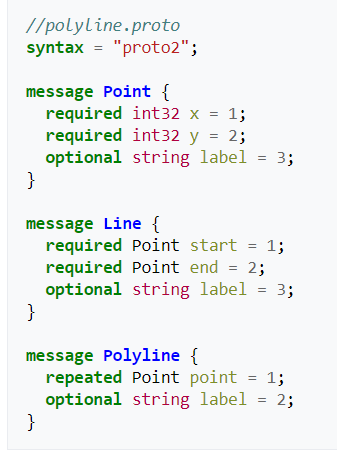
\includegraphics[width=60mm]{img/protobuf.PNG}
\end{figure}


\subsection{GFS - Google File System}
File system distribuito e fault-tolerant che memorizza e ritorna dati efficientemente. 
\begin{itemize}
    \item FS di archiviazione distribuito
    \item Fornisce chiamate POSIX di base uguali alla programmazione in locale (open, read, write, close)
    \item Consente a più client di accedere contemporaneamente
    \item Migliora disponibilità dei dati archiviando più copie in diverse macchine
    \item E' fault tolerant impiegando la ridondanza, ha molte copie dei file su macchine diverse
\end{itemize}

\begin{figure}[h]
\centering
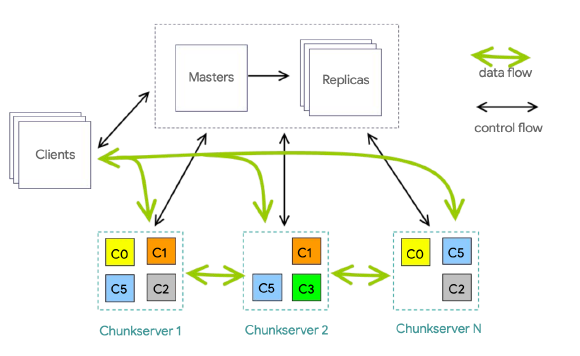
\includegraphics[width=90mm]{img/gfs.PNG}
\end{figure}
I client comunicano tramite control flow con il server master (anch'essi replicati). Quando un client vuole aprire un file chiede a uno dei master dove trovare il file, il master ridà una lista di locazioni dove i file risiedono. Siccome i file possono essere arbitrariamente grandi possono essere suddivisi in più chunk, ciascuno di questi frammenti è copiato in qualche chunkserver (il server master ad ex. dice al client che il suo file è diviso in due chunk e gli comunica dove trovare entrambi).
\bigbreak
Esistono due tipi di nodi: nodi master e nodi chunk. I chunk sono macchine server che conservano i file di dati chiamati appunto "chunk". I master sono macchine server che hanno competenze diverse: solitamente memorizzano i metadati associati ai chunk, come la posizione del file, le posizioni delle copie del chunk e quali processi stanno leggendo o scrivendo particolari chunk. Sono i server chunk ad aggiornare i master periodicamente per fare in modo che essi conservino metadati aggiornati. 
\bigbreak
I file sono divisi in chunk di dimensione fissa. Ogni chunk è identificato con un \textit{chunk handle} unico di 64bit assegnato dal master al momento della creazione del chunk. I chunk-server memorizzano i chunk nel disco locale. Per affidabilità, ogni chunk è replicato su molti chunkserver. Il master mantiene i metadati dei file, incluso namespace, informazioni di accesso, il mapping dai file ai chunk e la posizione corrente dei chunk. I client interagiscono con il master per operazioni su metadati, ma tutte le comunicazioni sui dati vanno direttamente al chunkserver. 

\subsection{GFS- Colossus}
L'implementazione originale di GFS ha ora più di 15 anni, adesso si è evoluto in Colossus. Per soddisfare nuovi requisiti, attualmente Google utilizza un nuovo codice tecnologie denominato Colossus:
\begin{itemize}
    \item utilizza la tecnologia Bigtable per l'archiviazione
    \item aumenta i limiti di dimensione dei file
    \item migliora la latenza
    \item diminuisce l'utilizzo dello spazio di archiviazione
\end{itemize}

\subsection{Bigtable}
Primo DB noSQL, cioè DB che rompono il paradigma SQL con tutte le sue proprietà. Bigtable semplifica molte assunzioni per riuscire a salvare mole di dati maggiori mantenendo bassa la latenza. Possiamo vederla come una grossa tabella di chiavi/valore. 
\bigbreak
Mappa ordinata distribuita e multidimensionale, cioè una tabella in cui in ciascuna riga c'è una chiave (identificatore) con un numero arbitrario di colonne. Data una riga e una colonna si possono recuperare le celle (plurale, c'è anche dimensione temporale). Le tabelle vengono divise in gruppi di record, di righe e ciascuno di essi diventa un tablet e viene allocato ad un tablet-server (ciascuno contiene circa 100 tablet). 
\bigbreak
Scala su migliaia di macchine (in un datacenter), fornisce la replica dei dati ed è costruito su GFS. 
\bigbreak
\noindent \textbf{Da Bigtable a Spanner}:
Bigtable non è male ma non garantisce atomicità delle transazioni (l'atomicità è garantita a livello di riga, se un client inserisce un record nella tabella, gli altri client non vedranno mai questa azione a metà: o vedono il file o non lo vedono). Non supporta le tabelle relazioni, per applicazioni che richiedono schemi complessi, Bigtable è difficile da usare.

\subsection{Spanner}
 Un nuovo sistema studiato e sviluppato per fornire maggiori garanzie rispetto a Bigtable rispetto alle transazioni e alla replica globale. Spanner è un DB distribuito multiversione (ci sono varie dimensioni temporali del dato)
 \begin{itemize}
     \item adotta un linguaggio SQL, ha tabelle schematizzate
     \item scala su molte macchine
     \item forti garanzie di consistenza
     \item possibilità di accedere ad una versione del DB in un certo periodo di tempo
 \end{itemize}
Spanner ha un sola istanza globale resa disponibile su ogni data center, ciasun data center ha una zona e un pool di master locali. IL dato è distribuito su server molto simili ai tabletserver di Bigtable chiamati Spanserver. Viene usato un protocollo Paxos che viene usato per decidere chi ottiene il lock (il locking avviene sul singolo tablet). 
\bigbreak
Spanner è un DB distribuito, scalabile sviluppato e rilasciato da Google. Al più alto livello di astrazione, è un DB che si frammenta in macchine che usano l'algoritmo Paxos. 
\subsection{F1}
Nella prima versione di Spanner molti aspetti opzionali di DB SQL sono stati tenuti fuori, questo per avere un DB engine che potesse essere applicato per molte applicazioni diverse. In realtà certe applicazioni avevano bisogno di dati complessi in termini di relazioni tra tabelle, per questo motivo si iniziò a lavorare ad un layer aggiuntivo per accedere a Spanner per aggiungere feature. In particolare si voleva un engine che mantenesse indici consistenti, che usasse data type più ricchi che le sole stringhe (Protocol Buffer) e un meccanismo per far evolvere lo schema del DB senza bloccare il servizio. 

\noindent F1:
\begin{itemize}
    \item Schemi relazionali (indici consistenti, più data type)
    \item Interfacce multiple (SQL, key/value, Mapreduce)
    \item Notifiche di modifica
\end{itemize}

\section{Processazione di informazione}
\subsection{Mapreduce}
Modello di programmazione per l'elaborazione e le generazione di grandi set di dati. Consente il calcolo parallelo di problemi della seguente forma 
\begin{equation}
    map: (k1,v1) \xrightarrow{} list(k2, v2) \\
    reduce (k2, list(v2)) \xrightarrow{} list(v2)
\end{equation}
Esempio: contare il numero di occorrenze di ogni parola in un ampio set di documenti: 
\begin{itemize}
    \item [-] Map function ridà un 1 simbolico per ogni parola
    \item [-] Reduce viene chiamato una volta per ogni parola, con la lista di valori associata ad essa
\end{itemize}

\begin{figure}[h]
\centering
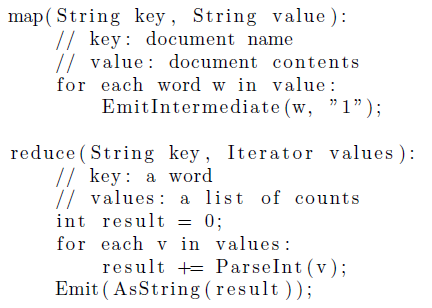
\includegraphics[width=90mm]{img/mapreduce.PNG}
\end{figure}
Il sistema esegue un importante passaggio aggiuntivo tra Map e Reduce chiamato SHUFFLE.
\begin{equation}
    map: (k1,v1) \xrightarrow{} list(k2, v2) \\
    shuffle: list(k2, v2) \xrightarrow{} (k2, list(v2)) \\
    reduce (k2, list(v2)) \xrightarrow{} list(v2)
\end{equation}

\subsection{FlumeJave}
Libreria Java per la scrittura di pipeline parallele ai dati. 

\subsection{MillWheel}

\chapter{Computing pervasivo}
"Le tecnologie più profonde sono quelle che scompaiono. Si intrecciano nel tessuto della vita quotidiana fino a quando non ne sono distinguibile". 
\bigbreak
I sistemi di pervasive computing sono sistemi distribuiti e mobili, l'elaborazione delle informazioni è stata interamente integrata all'interno di oggetti e attività di tutti i giorni. Chi utilizza ubiquitous computing aziona diversi sistemi nel corso di normali attività, senza quasi essere cosciente del fatto che questi macchinari stiano compiengo le proprie azioni e operazioni. 
\bigbreak
Il pervasive computing è un'area dell'informatica che ne coinvolge molti aspetti: reti, algoritmi, architetture, intelligenza artificiale. Nel pervasive computing non è solo importante avere un sistema di calcolo ma anche un sistema che risponda e si adatti all'ambiente che lo circonda. 
\begin{itemize}
    \item nodi non convenzionali
    \item adattività
    \item alta volatilità: sono molti nodi fragili che usano interfacce di comunicazione diverse, sono proni ad errori sia HW, di rete. La topologia di rete cambia spesso 
\end{itemize}
\noindent Problemi principali:
\begin{itemize}
    \item risorse limitate (energia, CPU, memoria)
    \item differenti tipi di interfaccia
    \item alta varianza nella connettività
    \item posizione variabile
\end{itemize}
\noindent Principali argomenti di ricerca
\begin{itemize}
    \item Networking (Mobile IP, reti ad hoc)
    \item Accesso mobile alle informazioni
    \item Gestione dei dati mobili (spazio-temporali, context-awareness)
    \item Positioning (localizzazione indoor o outdoor)
    \item Software
\end{itemize}
Esempi di sistemi pervasivi sono gli Smart Environment (Home, building, city) o sistemi per health-care. 

\section{IoT}
Particolare tipo di computing pervasivo. Il concetto rappresenta una possibile evoluzione dell'uso della rete internet: gli oggetti (le "cose") si rendono riconoscibili e acquisiscono intelligenza grazie al fatto di poter comunicare dati su se stessi e accedere ad informazioni aggregate da parte di altri[7]. Le sveglie suonano prima in caso di traffico, le scarpe da ginnastica trasmettono tempi, velocità e distanza per gareggiare in tempo reale con persone dall'altra parte del globo, i vasetti delle medicine avvisano i familiari se si dimentica di prendere il farmaco.
\bigbreak
Rete che non coinvolge solo utenti che eseguono applicazioni sui loro end.system ma anche un grande insieme di smart things che lavorano in modo autonomo, che interagiscono tra loro. 
\bigbreak
Perchè sono smart?
\begin{itemize}
    \item connessi ad internet (accesso remoto, invocazione di servizi)
    \item esecuzione di algoritmi per analizzare i dati e comprendere i contesti
    \item offre servizi contex-aware personalizzati
\end{itemize}
La guida autonoma ad ex. valuta il contesto con dei sensori e risponde in tempo reale riguardo cosa fare (mi fermo ad un semaforo?). 
\bigbreak
Le reti di sensori devono rispondere ad alcuni problemi (sono molti e proni ad errori). Posso utilizzare ad esempio delle reti ad albero anziché a stella per evitare la saturazione del gateway. 

\section{Acquisizione e gestione dei dati dai sensori}
Trasduttori: dispositivi che trasformano una forma di energia in un'altra forma di energia
\begin{itemize}
    \item Trasduttori di input - sensori (microfono)
    \item Trasduttori di output - attuatori (casse)
\end{itemize}
\bigbreak
\noindent \textbf{Sensori}
L'obbiettivo di un sensore è catturare un fenomeno fisico (inquinamento, temperatura, onde sonore) e digitalizzarlo (segnale elettrico). 
\bigbreak
Ci sono diversi tipi di sensori fisici:
\begin{itemize}
    \item Sensori di movimento (o inerziali): misurano accelerazioni, rotazione sui tre assi (accelerometri, sensori di gravità, giroscopi)
    \item Sensori ambientali: misurano parametri ambientali come temperatura, pressione, illuminazione, umidità (barometri, termometri)
    \item Sensori di posizione: misurano la posizione fisica di un device (magnetometri) 
\end{itemize}
Ci sono anche sensori virtuali: sono servizi e app che forniscono informazioni a clienti remoti (ci sono delle API, con un servizio REST, che ci ridanno le informazioni che vogliamo). 
\bigbreak
\noindent \textbf{Attuatori}
Gli attuatori sono particolari tipi di trasduttori, sono solitamente alimentati. Convertono energia in azione (moto, switch) a patto si ricevere un comando dal controllore del sistema (luci dimmerabili, volonte della macchina) 
\section{Comunicazione tra trasduttori}
Zigbee, ZWave e Thread sono tecnologie di rete con range limitati (10-20m), infatti le applicazioni sono in ambiente casalingo. Hanno data-rate limitati, ma tipicamente non hanno bisogno di comunicare dati enormi. Sono stati ideati per limitare il consumo di energia. La topologia di rete è mesh: ho dei device nella stanza che si presentano alla rete e partecipano. Il device si sposta e magari non riesce più a comunicare direttamente al gateway (in una topologia a stella c'è un punto centrale, il gateway, al quale si connettono tutti) e quindi comunicano con gli altri nodi, i nodi si aiutano a passare i messaggi che arriveranno comunque al gateway (scalabile, affidabile). Zigbee e Z-Wave non associano un indirizzo IP ai dispositivi, i dispositivi hanno un indirizzo interno alla rete. Thread ha l'obbiettivo di superare questo limite, rendendo ogni dispositivo IP-addressable. 
\end{document}